%% Adaptado a partir de :
%%    abtex2-modelo-trabalho-academico.tex, v-1.9.2 laurocesar
%% para ser um modelo para os trabalhos no IFSP-SPO

\documentclass[
    % -- opções da classe memoir --
    12pt,               % tamanho da fonte
    openright,          % capítulos começam em pág ímpar (insere página vazia caso preciso)
    %twoside,            % para impressão em verso e anverso. Oposto a oneside
    oneside,
    a4paper,            % tamanho do papel. 
    % -- opções da classe abntex2 --schwinn
    % Opções que não devem ser utilizadas na versão final do documento
    %draft,              % para compilar mais rápido, remover na versão final
    paginasA3,  % indica que vai utilizar paginas em A3 
    MODELO,             % indica que é um documento modelo então precisa dos geradores de texto
    TODO,               % indica que deve apresentar lista de pendencias 
    % -- opções do pacote babel --
    english,            % idioma adicional para hifenização
    brazil              % o último idioma é o principal do documento
    ]{ifsp-spo-inf-ctds} % ajustar de acordo com o modelo desejado para o curso


% ---
% Informações de dados para CAPA e FOLHA DE ROSTO
% ---
\titulo{PETINDER}

\renewcommand{\imprimirautor}{
\begin{tabular}{lr}
BRENDA OLIVEIRA DE SOUSA  & SP1851551 \\
CECÍLIA DUARTE GAMA & SP1852639 \\
EDUARDA BOMFIM DA CONCEIÇÃO & SP1852281 \\
FERNANDA APARECIDA FIGUEIREDO DA SILVA & SP1852124 \\
GABRIELA GONÇALVES MENDONÇA LINO & SP1850814 \\
GIOVANA PAZ PEDROZO & SP185089X \\
\end{tabular}
}


\disciplina{PDS - Prática de Desenvolvimento de Sistemas}

\preambulo{Trabalho apresentado à disciplina de Prática de Desenvolvimento de Sistemas do curso técnico em informática integrado ao ensino médio do Instituto Federal de São Paulo, como requisito principal para obtenção da aprovação na disciplina.}

\data{22 DE SETEMBRO DE 2021}

\renewcommand{\orientadorname}{Professor:}
\orientador{IVAN FRANCOLIN MARTINEZ}
\renewcommand{\coorientadorname}{Professor:}
\coorientador{LEONARDO ANDRADE MOTTA DE LIMA}


% ---


% informações do PDF
\makeatletter
\hypersetup{
        %pagebackref=true,
        pdftitle={\@title}, 
        pdfauthor={\@author},
        pdfsubject={\imprimirpreambulo},
        pdfcreator={LaTeX with abnTeX2 using IFSP model},
        pdfkeywords={abnt}{latex}{abntex}{abntex2}{IFSP}{\ifspprefixo}{trabalho acadêmico}, 
        colorlinks=true,            % false: boxed links; true: colored links
        linkcolor=blue,             % color of internal links
        citecolor=blue,             % color of links to bibliography
        filecolor=magenta,              % color of file links
        urlcolor=blue,
        bookmarksdepth=4
}
\makeatother
% --- 

% carregando aqui referencias quando utilizando BIBLATEX
\IfPackageLoaded{biblatex}{%
\addbibresource{referencias.bib}
\addbibresource{abntex2-doc-abnt-6023.bib}
}{}

% Início do documento
% ----
\begin{document}

% Retira espaço extra obsoleto entre as frases.
\frenchspacing 

% -- lista de pendencias gerada pelo todonotes
% -- altere opções do usepackage para remover na versão final....
\listoftodos
\todo[inline]{remover lista de todo da versão final...}
\newpage

% ----------------------------------------------------------
% ELEMENTOS PRÉ-TEXTUAIS
% ----------------------------------------------------------
\pretextual

% ---
% Capa
% ---
\imprimircapa

\newcounter{todocounter}
\newcommand{\todonum}[2][]
{\stepcounter{todocounter}\todo[#1]{\thetodocounter: #2}}
% ---

% ---
% Folha de rosto
% (o * indica que haverá a ficha bibliográfica)
% ---
\imprimirfolhaderosto
%\imprimirfolhaderosto*
% ---

% Quando registrado na biblioteca
%
% ---
% Inserir a ficha bibliografica
% ---

% Isto é um exemplo de Ficha Catalográfica, ou ``Dados internacionais de
% catalogação-na-publicação''. Você pode utilizar este modelo como referência. 
% Porém, provavelmente a biblioteca da sua universidade lhe fornecerá um PDF
% com a ficha catalográfica definitiva após a defesa do trabalho. Quando estiver
% com o documento, salve-o como PDF no diretório do seu projeto e substitua todo
% o conteúdo de implementação deste arquivo pelo comando abaixo:
%
% \begin{fichacatalografica}
%     \includepdf{fig_ficha_catalografica.pdf}
% \end{fichacatalografica}
\begin{fichacatalografica}
    \vspace*{\fill}                 % Posição vertical
    \hrule                          % Linha horizontal
    \begin{center}                  % Minipage Centralizado
    \begin{minipage}[c]{12.5cm}     % Largura
    
    \imprimirautor
    
    \hspace{0.5cm} \imprimirtitulo  / \imprimirautor. --
    \imprimirlocal, \imprimirdata-
    
    \hspace{0.5cm} \pageref{LastPage} p. : il. (algumas color.) ; 30 cm.\\
    
    \hspace{0.5cm} \imprimirorientadorRotulo~\imprimirorientador\\
    
    \hspace{0.5cm}
    \parbox[t]{\textwidth}{\imprimirtipotrabalho~--~\imprimirinstituicao,
    \imprimirdata.}\\
    
    \hspace{0.5cm}
        1. Palavra-chave1.
        2. Palavra-chave2.
        I. Orientador.
        II. Universidade xxx.
        III. Faculdade de xxx.
        IV. Título\\            
    
    \hspace{8.75cm} CDU 02:141:005.7\\
    
    \end{minipage}
    \end{center}
    \hrule
\end{fichacatalografica}
% ---



%Caso necessário
%% ---
% Inserir errata
% ---
\begin{errata}
Elemento opcional da \citeonline[4.2.1.2]{NBR14724:2011}. Exemplo:

\vspace{\onelineskip}


FERRIGNO, C. R. A. \textbf{Tratamento de neoplasias ósseas apendiculares com
reimplantação de enxerto ósseo autólogo autoclavado associado ao plasma
rico em plaquetas}: estudo crítico na cirurgia de preservação de membro em
cães. 2011. 128 f. Tese (Livre-Docência) - Faculdade de Medicina Veterinária e
Zootecnia, Universidade de São Paulo, São Paulo, 2011.

\begin{table}[htb]
\center
\footnotesize
\begin{tabular}{|p{1.4cm}|p{1cm}|p{3cm}|p{3cm}|}
  \hline
   \textbf{Folha} & \textbf{Linha}  & \textbf{Onde se lê}  & \textbf{Leia-se}  \\
    \hline
    1 & 10 & auto-conclavo & autoconclavo\\
   \hline
\end{tabular}
\end{table}

\end{errata}
% ---

%Obrigatório para trabalhos com bancas oficiais
%\input{pre-aprovacao}

% ---- opcionais 
% ---
% Dedicatória
% ---
\begin{dedicatoria}
   \vspace*{\fill}
   \centering
   \noindent
   \textit{ Este trabalho é dedicado às nossas famílias por nos apoiarem nos momentos\\ bons e ruins e a nós, integrantes da equipe TI TI TI, pela bravura de \\
   completar mais uma etapa.} 
   
   \vspace*{\fill}
   

\end{dedicatoria}
% ---
% ---
% Agradecimentos
% ---
\begin{agradecimentos}
\todonum[inline]{colocar seus agradecimentos}
Os agradecimentos principais são direcionados à Gerald Weber, Miguel Frasson,
Leslie H. Watter, Bruno Parente Lima, Flávio de Vasconcellos Corrêa, Otavio Real
Salvador, Renato Machnievscz\footnote{Os nomes dos integrantes do primeiro
projeto abn\TeX\ foram extraídos de
\url{http://codigolivre.org.br/projects/abntex/}} e todos aqueles que
contribuíram para que a produção de trabalhos acadêmicos conforme
as normas ABNT com \LaTeX\ fosse possível.

Agradecimentos especiais são direcionados ao Centro de Pesquisa em Arquitetura
da Informação\footnote{\url{http://www.cpai.unb.br/}} da Universidade de
Brasília (CPAI), ao grupo de usuários
\emph{latex-br}\footnote{\url{http://groups.google.com/group/latex-br}} e aos
novos voluntários do grupo
\emph{\abnTeX}\footnote{\url{http://groups.google.com/group/abntex2} e
\url{http://abntex2.googlecode.com/}}~que contribuíram e que ainda
contribuirão para a evolução do \abnTeX.

\end{agradecimentos}
% ---
% ---
% Epígrafe
% ---
\begin{epigrafe}
    \vspace*{\fill}
    \begin{flushright}
        \textit{``Não vos amoldeis às estruturas deste mundo, \\
        mas transformai-vos pela renovação da mente, \\
        a fim de distinguir qual é a vontade de Deus: \\
        o que é bom, o que Lhe é agradável, o que é perfeito.''\\
        (Bíblia Sagrada, Romanos 12, 2)}
    \end{flushright}
\end{epigrafe}
% ---

% -- resumo obrigatório
% ---
% RESUMOS
% ---

% resumo em português
\setlength{\absparsep}{18pt} % ajusta o espaçamento dos parágrafos do resumo
\begin{resumo}
\label{resumo}
Este documento, contendo textos, arquivos e imagens, foi formulado de modo a detalhar o desenvolvimento da aplicação \textit{web} PETINDER, solicitado pela disciplina de \ac{PDS}. O conceito deste projeto está relacionado ao crescente problema social de abandono animal, mesmo considerando que no início da pandemia de \gls{COVID-19} os números de adoção tenham aumentado no Brasil, o dilema
persistiu e a taxa de animais em situação de desamparo voltou a subir. A plataforma PETINDER visa facilitar o processo de adoção conectando de forma dinâmica doador e adotante. O usuário que optar pela nossa aplicação irá desfrutar de filtros de preferência quanto a características do animal que deseja adotar, uma listagem de animais cadastrados no sistema, poderá interagir com os perfis disponíveis (por meio do \gls{Miau-dorei} e do \gls{Des-au-gostei}, que funcionam respectivamente como nossas opções de gostei e não gostei) entre outras funções, como \textit{chat}, localização e \gls{Match}, que serão detalhadas ao longo da documentação.
%Segundo a ABNT(2003, 3.1-3.2), o resumo deve ressaltar o contexto, o objetivo, o método,os resultados e as conclusões do documento (portanto deve ser escrito por ultimo). A ordem e a extensão destes itens dependem do tipo de resumo (informativo ou indicativo) e do  tratamento que cada item recebe no documento original. O resumo \textbf{deve ter um paragrafo único} e deve \textbf{ter entre 150 e 500 palavras para trabalhos acadêmicos ou entre 100 e 250 para artigos de periódicos}. O resumo deve ser  precedido da referência do documento, com exceção do resumo inserido no  próprio documento. (\ldots) As palavras-chave devem figurar logo abaixo do resumo, antecedidas da expressão \textbf{Palavras-chave}:, separadas entre si por ponto e finalizadas também por ponto.

 \textbf{Palavras-chaves}: Adoção. Animais. Aplicação web. Doação.
\end{resumo}

% resumo em inglês
\begin{resumo}[Abstract]
 \begin{otherlanguage*}{english}
   This document, containing texts, files and images, was formulated in order to detail the development of the web application PETINDER, requested by the discipline of \ac{PDS}. The concept of this project is related to the growing social problem of animal abandonment, even considering that at the beginning of the \gls{COVID-19} pandemic the adoption numbers increased in Brazil, the problem persisted, and the abandonment rate rose again. The PETINDER platform aims to facilitate the adoption process by dynamically connecting donor and adopter. The user who chooses our application will be able to use preferential filters regarding the characteristics of the animal he wishes to adopt, a list of animals registered in the system, he will be able to interact with the available profiles liking or ignoring the animal's profile, among other functions such as chat, localization and \gls{Match}, which will be detailed throughout the documentation.


   \vspace{\onelineskip}

   \noindent 
   \textbf{Keywords}: Adoption. Animals. Web aplication. Donation.
 \end{otherlanguage*}
\end{resumo}


% ---
% inserir lista de ilustrações
% ---
\pdfbookmark[0]{\listfigurename}{lof}
\listoffigures*
\cleardoublepage
% ---

% ---
% inserir lista de tabelas
% ---
\pdfbookmark[0]{\listtablename}{lot}
\listoftables*
\cleardoublepage
% ---

% ---
% inserir lista de quadros
% ---
\pdfbookmark[0]{\listofquadrosname}{loq}
\listofquadros*
\cleardoublepage
% ---

%% ---
% inserir lista de abreviaturas e siglas
% ATENCAO o SHARELATEX/OVERLEAF GERA O GLOSSARIO SOMENTE UMA VEZ
% CASO SEJA FEITA ALGUMA ALTERAÇÃO NA LISTA DE SIGLAS É NECESSARIO UTILIZAR A OPÇÃO :
% "Clear Cached Files" DISPONIVEL NA VISUALIZAÇÃO DOS LOGS 
% ---
% https://www.sharelatex.com/learn/Glossaries


\ifdef{\printnoidxglossary}{
    \printnoidxglossary[type=\acronymtype,title=Lista de abreviaturas e siglas,style=siglas]
    \cleardoublepage
}{}


%% ---
% inserir lista de símbolos
% ---
\begin{simbolos}
  \item[$ \Gamma $] Letra grega Gama
  \item[$ \Lambda $] Lambda
  \item[$ \zeta $] Letra grega minúscula zeta
  \item[$ \in $] Pertence
\end{simbolos}
% ---

\todo[inline]{Remover lista de simbolos se não for necessário}


% ---
% inserir o sumario
% ---
\pdfbookmark[0]{\contentsname}{toc}
\tableofcontents*
\cleardoublepage
% ---


% ----------------------------------------------------------
% ELEMENTOS TEXTUAIS
% ----------------------------------------------------------
\textual

% ----------------------------------------------------------
% Introdução
% ----------------------------------------------------------
\chapter[Introdução]{Introdução}
No Brasil temos muitos casos de abandonos de animais. Em 2019 o Instituto Pet Brasil realizou um levantamento a respeito de animais sob tutela de \ac{ONGs}, e chegaram ao resultado de mais de 170 mil animais. Desses, 96\% são cachorros e apenas 4\% são gatos. Além das \ac{ONGs} muitas pessoas resgatam animais que encontram na rua em situações de vulnerabilidade, levam para suas casas e fornecem lares temporários até encontrarem, então, uma família que possa oferecer todo cuidado que o animal necessita \cite{tutelaONG}.

O ano de 2020 foi marcado pela pandemia da \gls{COVID-19}, devido a isso, a população foi submetida a um período de quarentena obrigatória. Nos primeiros meses, com mais tempo em casa, os brasileiros recorreram a \ac{ONGs} em busca de companhia animal, aumentando os números de adoções \cite{adocao}.

O país foi afetado em diversas questões: econômica, social, política e culturalmente, causando, assim, uma reviravolta na vida de todos, inclusive dos animais. Novamente o índice de abandono cresce, e com alguns fatores como desemprego em grandes níveis, retorno de atividades presenciais, fim do auxílio emergencial, o cuidado dos amimais ficou inviável para alguns tutores \cite{abandono_pandemia}. 

Visando facilitar o processo de adoção, tanto para o adotante, como para o doador, a equipe TI TI TI decidiu por desenvolver um \textit{website} que atendesse às necessidades dos usuários, possibilitando a busca por um animal que combine com as premissas do adotante.

\section{Problema a ser solucionado}
Em 2013 a \ac{OMS} lançou uma nota que continha estimativas do número de animas vivendo nas ruas do Brasil, eram cerca de 20 milhões de cães e 10 milhões de gatos. Em cidades grandes como São Paulo e Rio de Janeiro há um cachorro a cada 5 habitantes, e 10\% destes não tem um lar.

Com o início da pandemia e confinamento brasileiro, as \ac{ONGs} passaram a reportar um aumento na procura de adoção de cães e gatos. Segundo o médico veterinário que é gerente de vigilância do \ac{CCZ} do Distrito Federal, Rodrigo Menna Barreto, o número de adoções de animais registrados pelo órgão entre janeiro e setembro de 2020 foi maior que o dobro registrado em todo o ano anterior.

Infelizmente essa rara notícia boa não durou, quando a pandemia passou a viver seu pior momento no Brasil com crise social e econômica, muitos dos animais voltaram ao seu destino anterior sendo abandonados ou devolvidos por famílias que alegaram falta de condições financeiras ou psicológicas para cria-los, além daqueles que os abandonavam por medo de ter \gls{COVID-19} por transmissão de cães e/ou gatos (uma informação comprovada falsa). Isso levou a \ac{ONGs} superlotadas e recordes de abandono.

\section{Justificativa}
Diariamente ao sairmos de nossas casas, cenas de cães e gatos abandonados são muito comuns, principalmente em centros urbanos, onde reside a maior parte da população. Na pandemia é notável que essas cenas acabaram ficando cada vez mais frequente, tornando a reflexão acerca do tema um tanto relevante.

De acordo com dados da \gls{AMPARA}, cerca de 60\% a 70\% de animais foram abandonados, entre julho de 2020 e fevereiro de 2021 (em comparação com 2019). Um dos muitos motivos para tal estimativa é a dificuldade financeira, e adoção por impulso durante o período de quarentena \cite{abandono}.

Em vista de tais dados, nossa equipe se sensibilizou com a causa e decidiu criar um projeto que realize a adoção de cães e gatos de forma prática e efetiva, contribuindo, dessa forma, com a diminuição dos números de abandonos, de maneira consciente e solidária.

\section{Objetivos}

A equipe TI TI TI desenvolveu o \textit{website} PETINDER visando prover para os usuários da plataforma um local seguro onde possa acontecer a conexão entre animal e adotante. Temos como objetivo também auxiliar na queda dos números de animais em situação de rua e ajudar cães e gatos a encontrarem novos lares onde possam receber proteção e afeto.

O projeto tem como objetivos específicos:

\begin{itemize}
\item Facilitar o processo de adoção de cães e gatos;
\item Oferecer uma plataforma segura e intuitiva para o usuário;
\item Colaborar com a diminuição do número de animais abandonados do país.
\end{itemize}

% ---
% Capitulo de revisão de literatura
% ---
\chapter{Revisão da Literatura}
A revisão da literatura é a etapa do trabalho em que se reúne as fontes de pesquisa que vão fornecer embasamento teórico para o trabalho.

Além disso, serve para dialogar com essas referências e aplicar seus conceitos no tema da monografia.

Portanto, é na revisão da literatura onde deve-se apresentar um levantamento bibliográfico acerca do assunto que será tratado na monografia, com escopo definido e uma análise crítica sobre os autores selecionados. 

%Todos trabalhos devem possuir a revisão de literatura onde são abordados os estudos feitos com base da literatura (livros, artigos acadêmicos, publicações em periódicos), todos elementos devem ser referenciados por citações.

%Não são abordados aqui itens técnicos que normalmente são vistos em disciplinas anteriores do curso (UML, banco de dados, metodologias de gerenciamento de projeto etc...)

\section{Assunto X}

\chapter{Descrição funcional da aplicação}
% Falar das funcionalidades da aplicacao, das partes interessadas, e dos concorrentes (incluir tabela de comparacao)

\section{Casos de uso}
% Descricao e diagrama

\input{desenvolvimento/texto-modelagem}
% ----------------------------------------------------------
% Finaliza a parte no bookmark do PDF
% para que se inicie o bookmark na raiz
% e adiciona espaço de parte no Sumário
% ----------------------------------------------------------
\phantompart

% ----------------------------------------------------------
% ELEMENTOS PÓS-TEXTUAIS
% ----------------------------------------------------------
\postextual
% ----------------------------------------------------------

% ----------------------------------------------------------
% Referências bibliográficas
% ----------------------------------------------------------
% quando não esta utilizando biblatex tem que carregar as referencias aqui
\IfPackageLoaded{biblatex}{}{%
\bibliography{referencias,exemplos/abntex2-doc-abnt-6023}
}

% ----------------------------------------------------------
% Glossário
% ----------------------------------------------------------
%
%
\ifdef{\printnoidxglossary}{
    \addcontentsline{toc}{chapter}{GLOSSÁRIO}
    \printnoidxglossary[style=glossario]
    %\printglossaries
}{}

% ----------------------------------------------------------
% Apêndices
% Documentos gerados pelo próprio autor
% ----------------------------------------------------------
% ---
% Inicia os apêndices
% ---
\begin{apendicesenv}

\partapendices

% Documento Proposta Inicial na pasta "apendices"
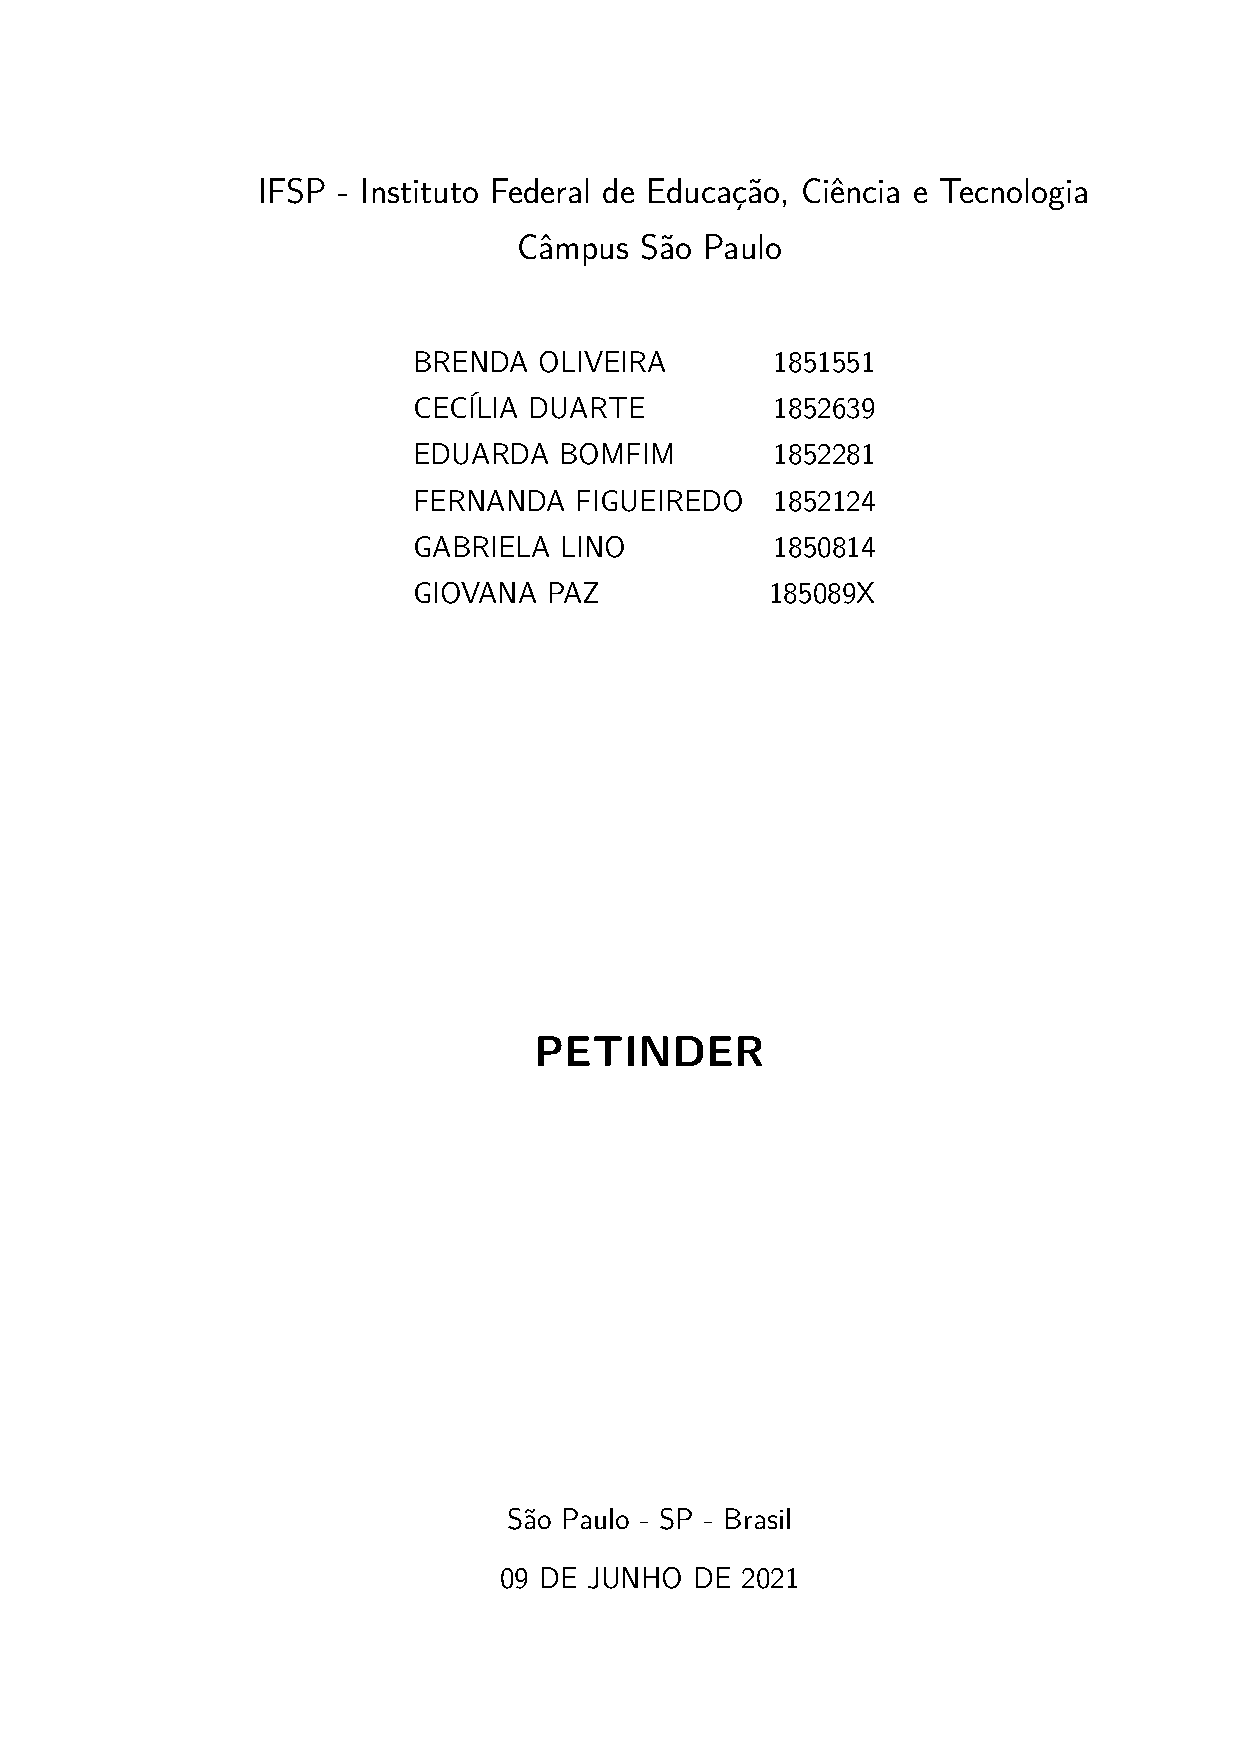
\includepdf[pages=1,scale=0.7,frame=true,pagecommand=\chapter{Proposta Inicial}\label{propostainicial-pdfpages}]{apendices/PropostaInicial.pdf}

\includepdf[pages=2-14,scale=0.7,frame=true,pagecommand={}]{apendices/PropostaInicial.pdf}

% Documento Prova Conceitual na pasta "apendices"
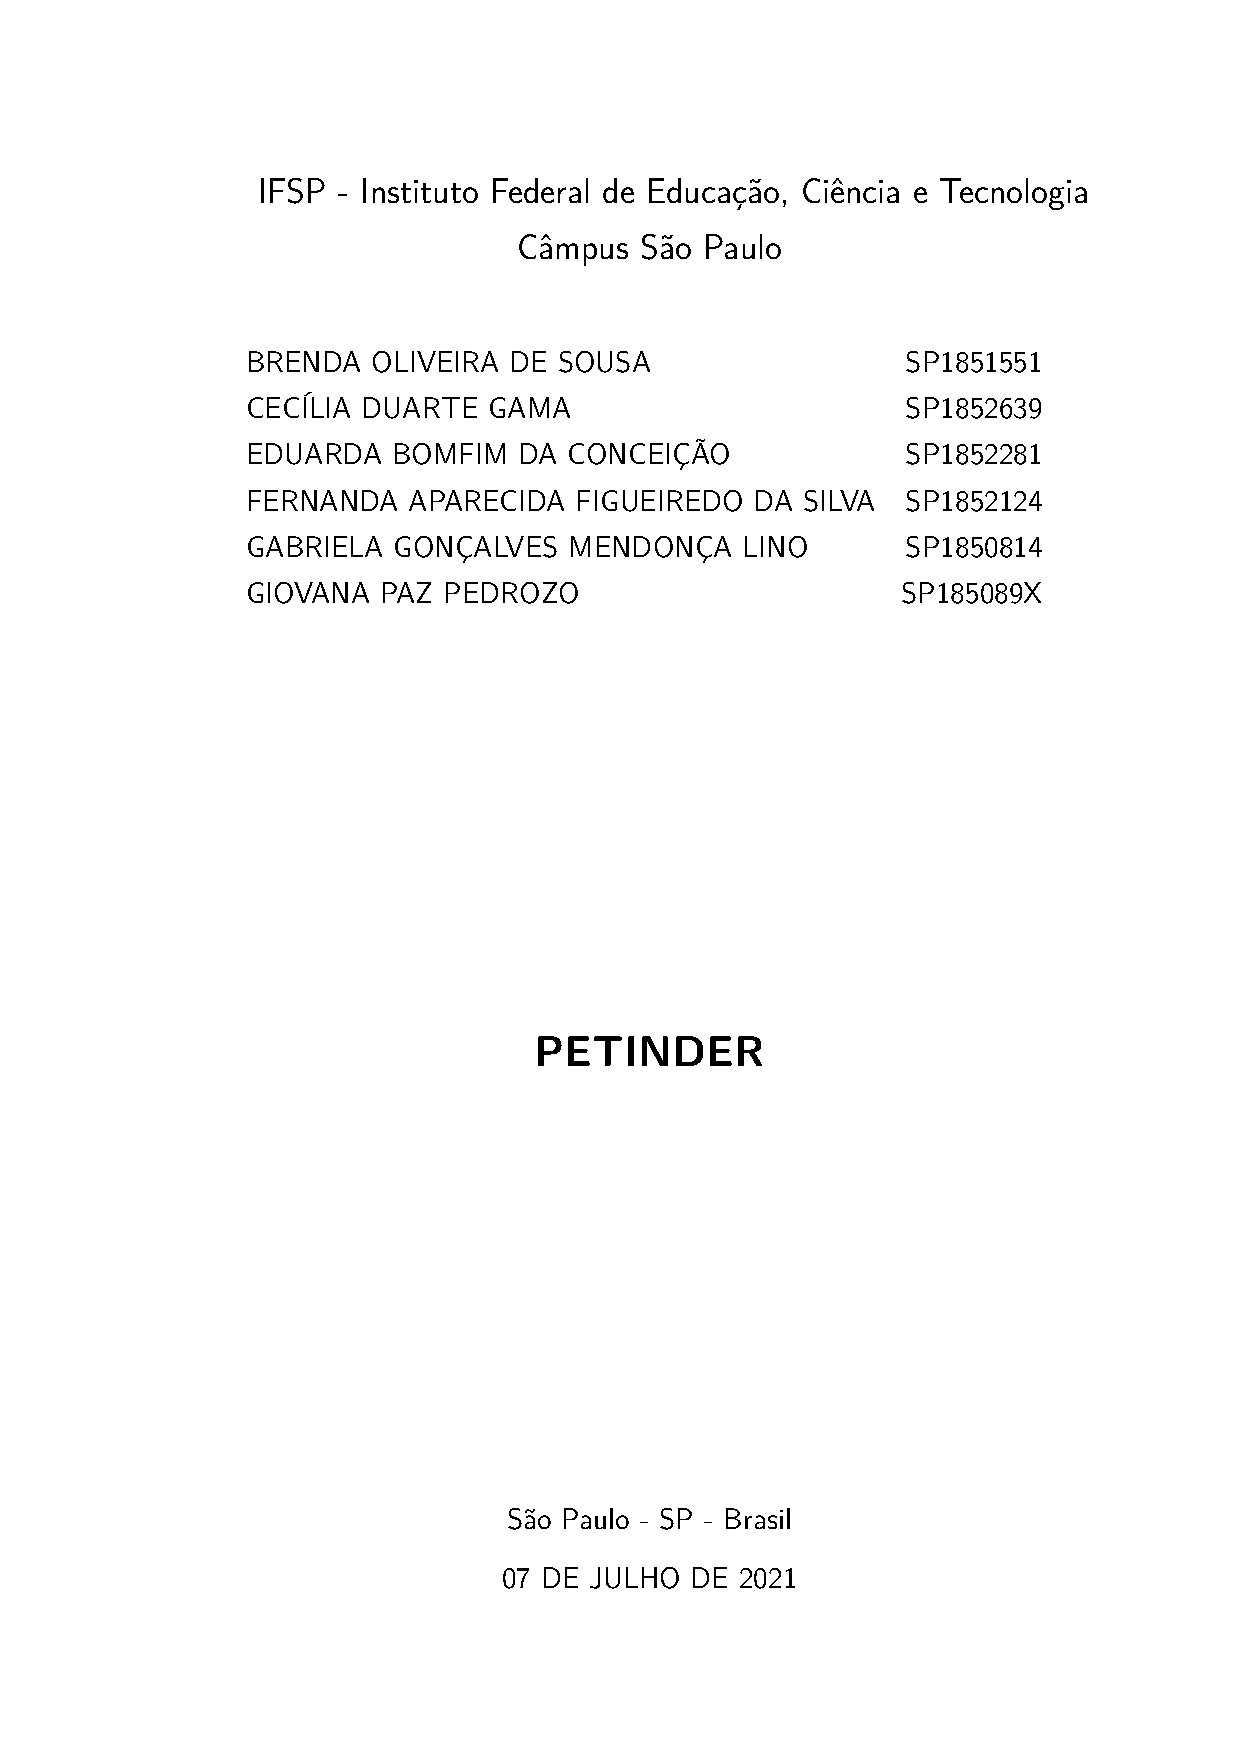
\includepdf[pages=1,scale=0.7,frame=true,pagecommand=\chapter{Prova Conceitual}\label{provaconceitual-pdfpages}]{apendices/ProvaConceitual.pdf}

\includepdf[pages=2-10,scale=0.7,frame=true,pagecommand={}]{apendices/ProvaConceitual.pdf}

%Imagens do Cronograma Mensal
\chapter{Cronogramas Mensais}
\centering
\label{Cronogramas-mensais}
%MAIO------------------------
\begin{figure}[!htbp]
\begin{flushleft}
  \section{Maio}  
\end{flushleft}
    \centering
    \caption{Cronograma Maio}
    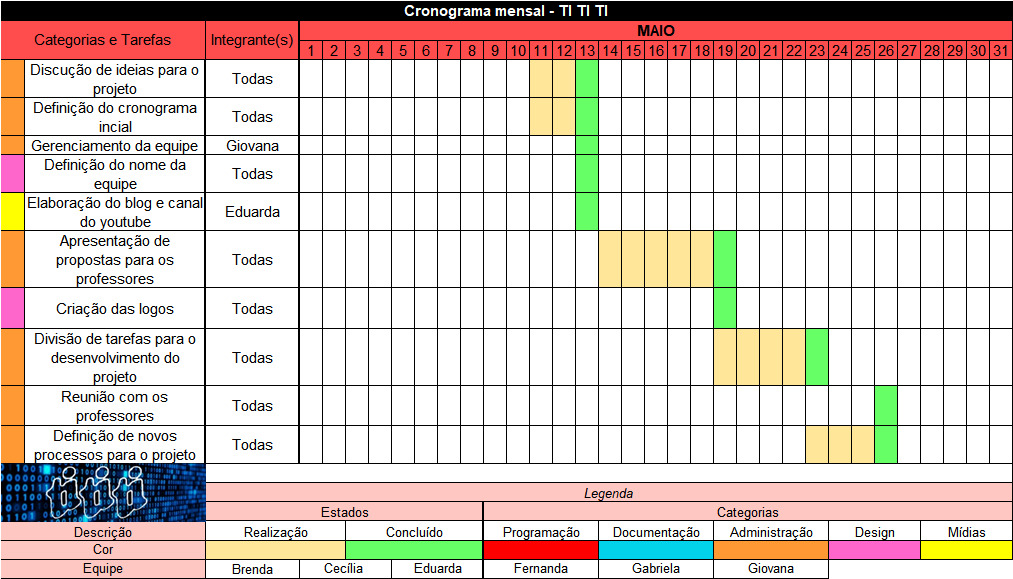
\includegraphics[scale=0.5,angle=90,pagecommand={}\label{cronograma-maio}]{imagens/CronogramaMAIO.jpeg}
    \fonte{Elaborado pelos autores}
\end{figure}

%JUNHO------------------------
\begin{figure}[!htbp]
\begin{flushleft}
    \section{Junho - Parte 1}
\end{flushleft}
    \centering
    \caption{Cronograma Junho (I) }
    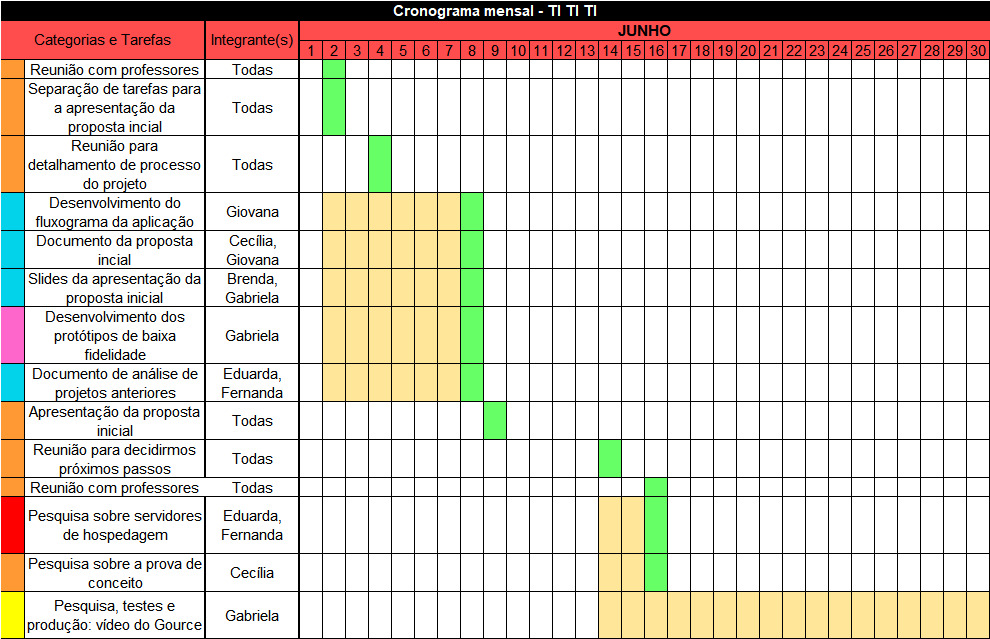
\includegraphics[scale=0.6,angle=90,pagecommand={}\label{cronograma-junho1}]{imagens/CronogramaJUNHO_01.jpeg}
    \fonte{Elaborado pelos autores}
\end{figure}

%----------
\begin{figure}[!htbp]
\begin{flushleft}
    \section{Junho - Parte 2}
\end{flushleft}
    \centering
    \caption{Cronograma - Junho (II)}
    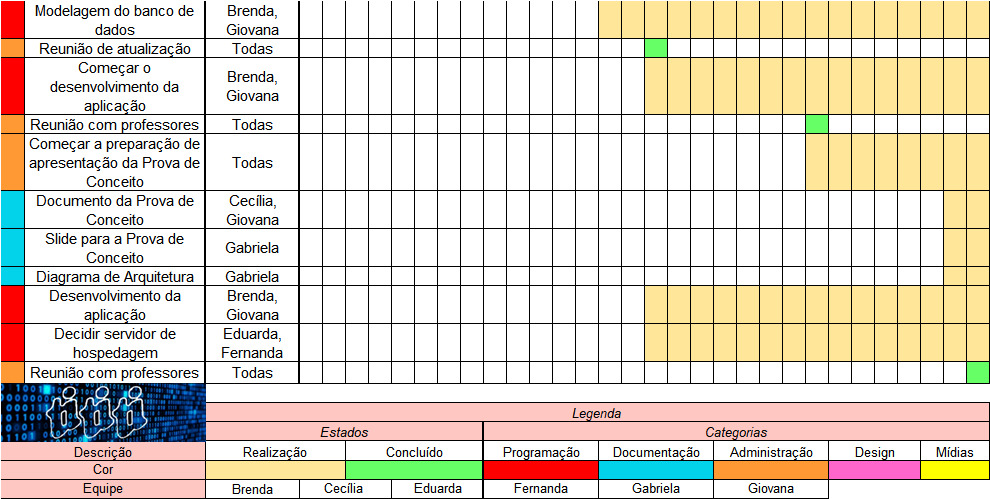
\includegraphics[scale=0.6,angle=90,pagecommand={}\label{cronograma-junho2}]{imagens/CronogramaJUNHO_02.jpeg}
    \fonte{Elaborado pelos autores}
\end{figure}

%JULHO------------------------
\begin{figure}[!htbp]
\begin{flushleft}
    \section{Julho - Parte 1}
\end{flushleft}
    \centering
    \caption{Cronograma - Julho (I)}
    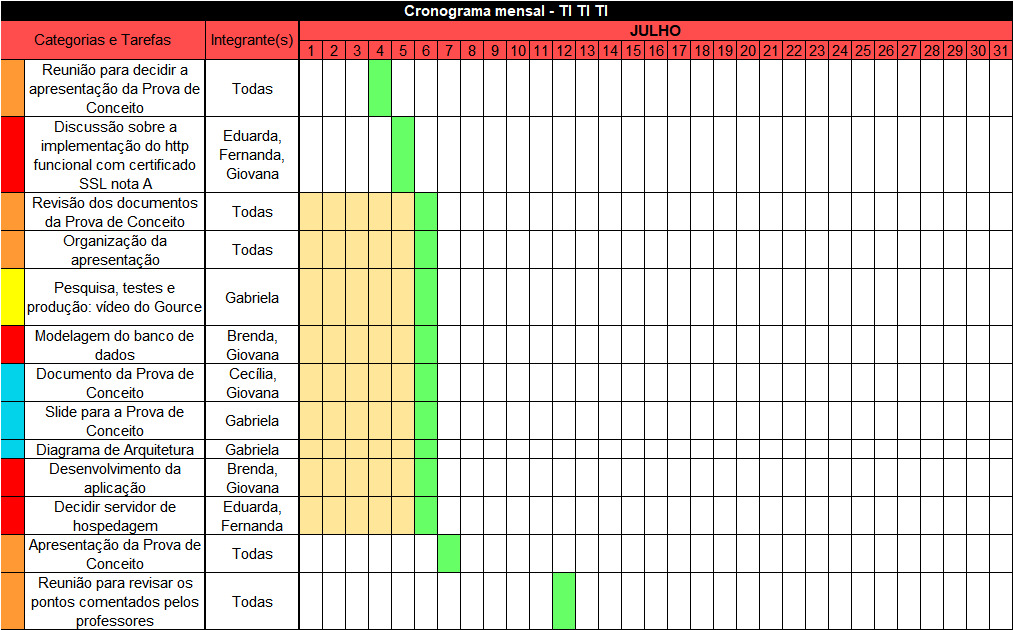
\includegraphics[scale=0.6,angle=90,pagecommand={}\label{cronograma-julho2}]{imagens/CronogramaJULHO_01.jpeg}
    \fonte{Elaborado pelos autores}
\end{figure}

%----------
\begin{figure}[!htbp]
\begin{flushleft}
    \section{Julho - Parte 2}
\end{flushleft}
    \centering
    \caption{Cronograma - Julho (II)}
    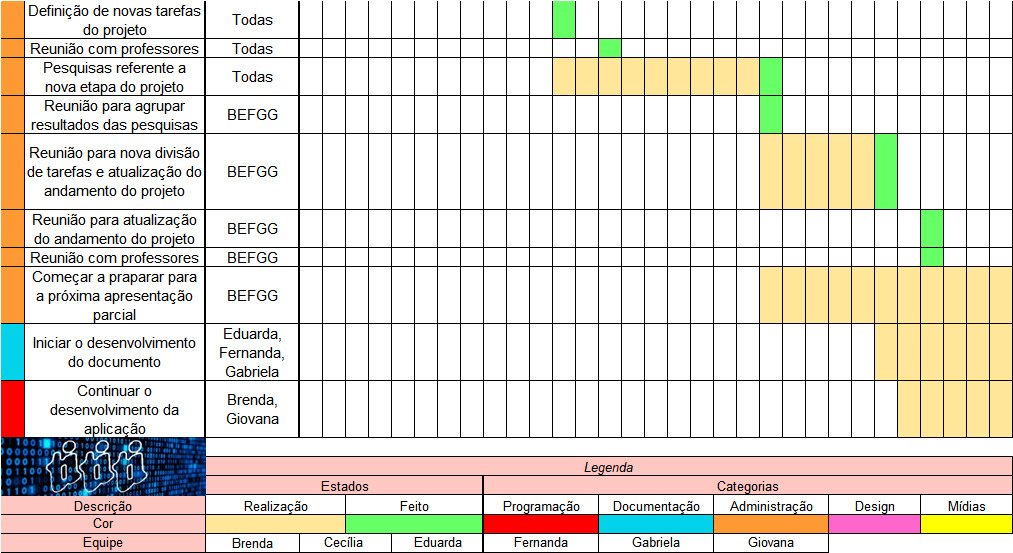
\includegraphics[scale=0.6,angle=90,pagecommand={}\label{cronograma-julho2}]{imagens/CronogramaJULHO_02.jpeg}
    \fonte{Elaborado pelos autores}
\end{figure}

%AGOSTO------------------------
\begin{figure}[!htbp]
\begin{flushleft}
    \section{Agosto}
\end{flushleft}
    \centering
    \caption{Cronograma - Agosto}
    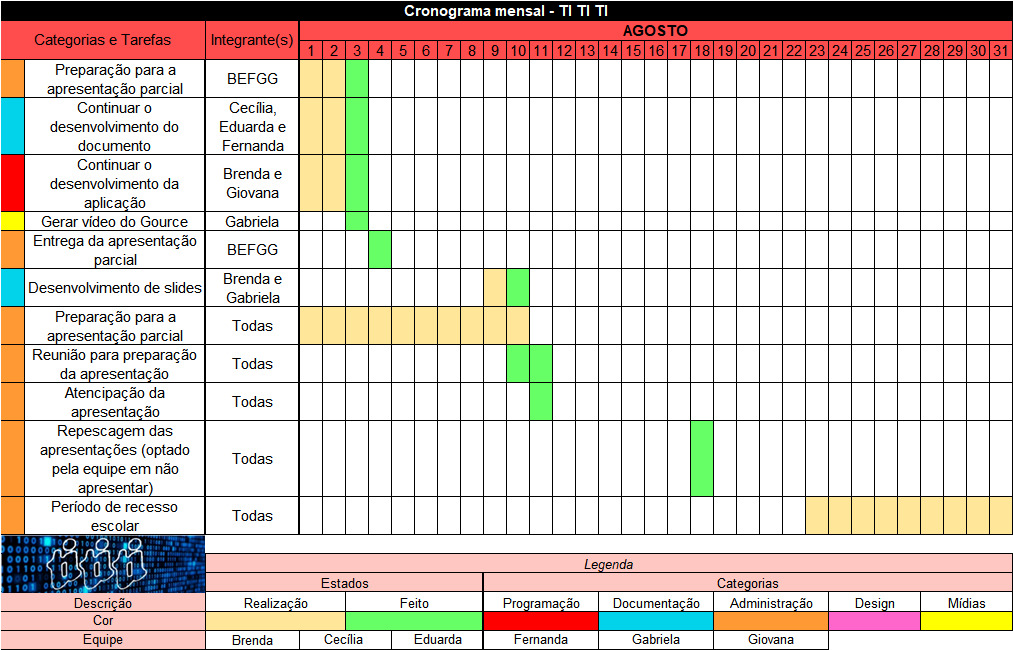
\includegraphics[scale=0.6,angle=90,pagecommand={}\label{cronograma-agosto}]{imagens/CronogramaAGOSTO.jpeg}
    \fonte{Elaborado pelos autores}
\end{figure}

%SETEMBRO------------------------
\begin{figure}[!htbp]
\begin{flushleft}
    \section{Setembro}
\end{flushleft}
    \centering
    \caption{Cronograma - Setembro}
    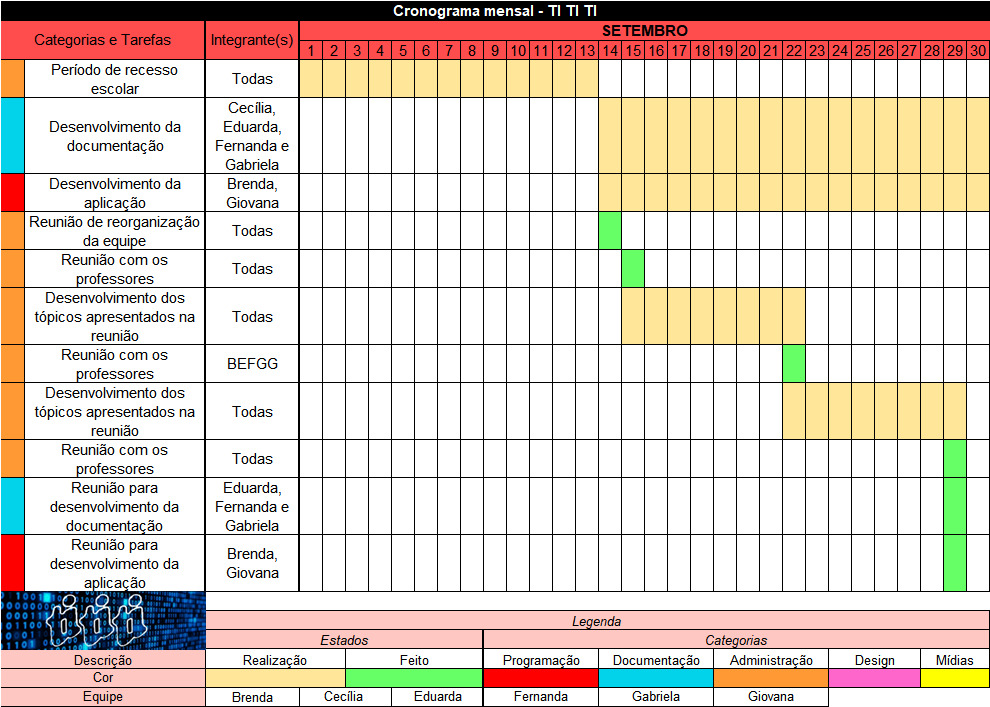
\includegraphics[scale=0.6,angle=90,pagecommand={}\label{cronograma-setembro}]{imagens/CronogramaSETEMBRO.jpeg}
    \fonte{Elaborado pelos autores}
\end{figure}
%------------------------

%Publicação do blog
\chapter{Publicações do blog}
\label{publicacoes-blog}
\begin{flushleft} %para alinhar à esquerda
    \section{Semana 01 - 12/05 até 18/05}


Nesta primeira semana nós nos reunimos e realizamos uma reunião com a participação de todas as integrantes para abordar e desenvolver os seguintes temas:
 \newline
- Explicamos sobre o que o projeto PETINDER (desenvolvido nas disciplinas anteriores de \ac{PJI} e \ac{TDS}) se tratava para as duas novas integrantes que não tinham afinidade com o tema, e pensamos juntas sobre melhorias a serem feitas nele;
 \newline
 
- Discutimos sobre novas ideias que poderiam se tornar tema do projeto;
  \newline
- Discutimos nomes que se encaixariam nessas novas ideias;
  \newline
- Definimos o nome da equipe;
  \newline
- Criamos a pasta do projeto no repositório da escola;
  \newline
- Definimos a gerente da nossa equipe.
\newline
\end{flushleft}
\begin{flushleft}
 \section{Semana 02 - 19/05 até 25/05}
 Nesta semana nós realizamos a primeira pré-apresentação de temas para os professores 

Antes disso fizemos uma reunião por video-chamada para filtrar os possíveis temas de projeto que tínhamos (7 que criamos na reunião da semana anterior)

Desses 7 temas apresentamos os únicos 2 que conseguimos pensar em processos: o Petinder e um aplicativo de auxílio para  estudo para vestibular

A integrante do grupo (Gabriela) fez um logo com o nome da equipe e a integrante (Brenda) fez uma conta no \gls{Instagram} para o projeto

Em uma segunda reunião durante esta semana nós dividimos as seguintes tarefas entre nossas integrantes:

1- Checar aplicativos semelhantes ao PETINDER 

2- Checar aplicativos de namoro

3- Comparar projetos semelhantes no repositório 

4- Revisar protótipos de baixa fidelidade 

5- Revisar os casos de uso do ano passado

6- Melhorar as entidades dos usuários

Planejamos uma reunião em breve para discutir os resultados das pesquisas

\gls{Instagram} do PETINDER: @petinder\_ti

\end{flushleft}
\begin{flushleft}
 \section{Semana 03 - 26/05 até 01/06}
  Nesta semana nosso grupo continuou focando no desenvolvimento da proposta do sistema PETINDER

Apresentamos em reunião de grupo na quarta-feira passada (26/05/21) os resultados das nossas pesquisas individuais (tarefas distribuídas na semana anterior) para todas e pensamos em mais processos que poderiam ser implantados e verificamos se eles eram válidos em apresentação para os professores 

A integrante do grupo (Giovana) realizou a inclusão do documento equipe.yaml no repositório
\end{flushleft}
\begin{flushleft}
 \section{Semana 04 - 02/06 até 08/06}
 Nesta semana nosso grupo fez quatro reuniões para discutir os próximos passos quanto ao projeto.

Na primeira definimos as tecnologias que serão utilizadas para desenvolver o projeto.

Na segunda a equipe analisou os protótipos de baixa fidelidade.

Na terceira reunião realizamos a divisão de tarefas que seguiremos ao longo do ano (sempre levando em consideração a necessidade de manter todas atualizadas sobre todos os avanços e ofertar ajuda quando aparecerem dificuldades ou dúvidas), participamos também da aula no dia 02/06 e apresentamos os avanços que tínhamos até aquele momento, anotamos todas as observações e críticas e discutimos sobre como prosseguir deste ponto.

Nós também separamos a equipe para realizar a documentação para a apresentação que ocorrerá nesta quarta-feira 09/06

Documentação da proposta inicial (Giovana)

Slides (Brenda e Gabriela)

Análise de propostas anteriores (Eduarda e Fernanda)

Nossa quarta reunião (08/06) aconteceu para que todas acompanhassem o progresso dessas atividades e para que pudéssemos treinar para a próxima apresentação

A integrante Giovana subiu o esqueleto das pastas no repositório.
\end{flushleft}
\begin{flushleft}
 \section{Semana 05 - 09/06 até 15/06}
  Nesta semana nós realizamos 2 reuniões 

A primeira na quarta-feira passada (08/06) para treinarmos as falas para a apresentação da proposta inicial antes da reunião com a turma e os professores

A segunda reunião foi nesta segunda-feira (14/06), onde nós discutimos sobre quais seriam os próximos passos em relação ao projeto

Voltamos para a área de pesquisa com o objetivo de reunir informações sobre os seguintes tópicos:

Pesquisar sobre o nicho que nossa aplicação se encaixa, pesquisar sobre a prova de conceito, pesquisar sobre o funcionamento do \gls{Gource} e sobre o servidor de hospedagem

Também pretendemos começar a modelar o banco de dados nesta semana

Nós indicamos o aplicativo \gls{Loom} para gravar o vídeo de proposta inicial dos grupos.
\end{flushleft}
\begin{flushleft}
 \section{Semana 06 - 16/06 até 22/06}
  Nesta semana nós fizemos uma reunião no \gls{Discord} para discutir os próximos passos em relação ao projeto, estamos reunindo informações e nos preparando para apresentação da prova de conceitos.

O vídeo da proposta inicial já está disponível em nosso canal no \gls{YouTube}.

Durante a aula de quarta-feira apresentamos a primeira versão do modelo de banco de dados, estamos revisando nossos requisitos funcionais, não-funcionais, regras de negócio e casos de uso, também estamos no processo de desenvolvimento dos modelos de classe e começando de fato o desenvolvimento da aplicação.
\end{flushleft}
\begin{flushleft}
 \section{Semana 07 - 23/06 até 29/06}
 Nesta semana nós realizamos 2 reuniões

Uma na quarta-feira (23/06) antes do encontro com os professores para atualizarmos todas as integrantes do grupo quanto ao andamento do projeto.

Nós preenchemos e colocamos no \gls{Subversion} a tabela de notas referente ao primeiro bimestre.

O grupo revisou e produziu novos requisitos funcionais, não-funcionais, regras de negócio e casos de uso.

Produzimos o diagrama de arquitetura, estamos os revisando e pretendemos apresentar aos professores no próximo encontro.

Nossa segunda reunião (29/06) também foi para atualizações quanto ao andamento do projeto, essas foram as informações que compartilhamos:

Nós definimos o \gls{000Webhost} como servidor de hospedagem para nossa aplicação.

Estamos pesquisando formas gratuitas para conseguir o certificado \ac{HTTPS}, \ac{SSL} e um \gls{Hostname}.

As telas que temos foram internacionalizadas, agora elas podem ser exibidas em inglês e português. 

Quanto a integração das telas com o banco de dados: conseguimos rodar uma versão teste, avanços futuros também serão relatados.

Também estamos avançando com o script do banco de dados e iniciamos o relatório e os slides para apresentação da prova de conceitos.
\end{flushleft}
\begin{flushleft}
 \section{Semana 08 - 30/06 até 06/07}
  Nesta semana nós aceleramos o andamento do projeto para a apresentação da \ac{POC}.

Nós nos deparamos com alguns problemas ao longo da semana relacionados ao servidor de hospedagem e certificado \ac{SSL}, testamos o \gls{000Webhost} com um domínio próprio e o \ac{SSL} não deu um retorno, testamos a aplicação no \gls{Heroku} porém o certificado \ac{SSL} emitido foi um com nota b. Finalmente hospedamos a aplicação na azure e o certificado \ac{SSL} veio com nota a.

Temos o relatório e os slides para a apresentação da \ac{POC} prontos.

A comunicação cliente-servidor e banco esta concluída, assim como o diagrama de arquitetura.

Nosso grupo usou o \gls{Discord} diversas vezes para se reunir, as integrantes se apoiaram bastante para conseguir resultados positivos.

Uma dica para os próximos alunos nessa matéria: pesquisem todas as alternativas que o \ac{IFSP} fornece de graça, com o \gls{GitHub} no pacote estudantil nós temos acesso a muitas opções (nomes de domínio de graça, contas na azure e \gls{Heroku}, entre outros), escolham o melhor servidor para a aplicação de vocês e aprendam como usar, leiam as instruções dos documentos que os professores orientadores fornecem e sigam a partir deste ponto.
\end{flushleft}
\begin{flushleft}
 \section{Semana 09 - 07/07 até 13/07}
 Nesta semana nós apresentamos a \ac{POC}.

Aqui vai um tutorial para as turmas futuras: durante a apresentação da prova de conceitos você precisa ter os slides (o nosso continha as tecnologias que estamos usando, o diagrama de arquitetura do sistema e os problemas que enfrentamos enquanto desenvolvíamos o sistema até o ponto atual) e a aplicação funcionando em algum servidor de hospedagem.

Trabalhem com esse diagrama de arquitetura pelo menos durante 2 reuniões com os professores, isso irá ajudar vocês a o desenvolver mais corretamente.

Vocês também irão precisar apresentar a aplicação. Atenção nisso, vocês precisam demonstrar que as tecnologias funcionam, vocês não precisam de um processo funcionando 100\%, só precisam provar que tudo que citaram que iriam usar pode realmente funcionar. 

Sejam atenciosos com isso, coloquem uma parte de todas as tecnologias que vocês falaram que iriam usar nessa apresentação.

Também não esquecem de postar o vídeo da aderência da aplicação no \gls{YouTube} ANTES da apresentação, isso irá custar pontos ao grupo.

Nesta semana nós fizemos apenas uma reunião, dividimos tarefas para reunir documentos e informações para a primeira versão da documentação final, todas as integrantes estavam presentes e estamos mantendo todas atualizadas sobre cada avanço no projeto.
\end{flushleft}
\begin{flushleft}
 \section{Semana 10 - 14/07 até 20/07}
 Realizamos uma reunião dia 14/07 para redistribuir tarefas relacionadas ao projeto e reunir mais informações sobre os próximos passos que temos que tomar.

Estamos recolhendo informações para nos prepararmos para iniciar a documentação da primeira versão da entrega final do projeto.

Seguimos revisando requisitos funcionais, não funcionais, regras de negócio e modelagem do banco, além de reunir as atas das reuniões anteriores, métricas do projeto e transcrevendo os cronogramas que usamos anteriormente.

Mantivemos as demais integrantes informadas pelo \gls{WhatsApp}.
\end{flushleft}
\begin{flushleft}
 \section{Semana 11 - 21/07 até 27/07}
 Nesta semana nós realizamos duas reuniões. A integrante Cecília não compareceu a nenhuma destas.

Na primeira revisamos os avanços da aplicação e das tarefas distribuídas anteriormente, tivemos um atraso em relação a documentação pois a mesma integrante que não compareceu as reuniões não entregou sua parte da documentação. 

A segunda reunião foi feita para redistribuição de tarefas, pretendemos ter avanços suficientes até a próxima semana.
\end{flushleft}
\begin{flushleft}
 \section{Semana 12 - 28/07 até 03/08}
 Nesta semana nós realizamos apenas uma reunião por chamada no \gls{Discord}, nela discutimos o avanço da aplicação e da documentação e redistribuímos tarefas relacionadas ao projeto.

Infelizmente a integrante Cecília não pode comparecer novamente, ela também não deu nenhum retorno quando tentamos contato pelo \gls{WhatsApp}. O grupo entrou em acordo quanto a tirar o nome dela da planilha de notas em decorrência dessa falta de comunicação e presença.

Estamos nos preparando para a próxima entrega, esperamos ter avanços significativos para apresentar.
\end{flushleft}
\begin{flushleft}
 \section{Semana 13 - 04/08 até 10/08}
 Nesta semana nossa equipe colocou ainda mais esforços na documentação para entrega parcial e no desenvolvimento da aplicação.

Criamos e postamos o vídeo do \gls{Gource} sobre a evolução do projeto até agora no nosso canal do \gls{YouTube}.

A integrante Cecília explicou que teve problemas pessoais durante as 3 semanas em que não manteve contato com o grupo, ela participou de uma parte do desenvolvimento do documento para entrega parcial.

Tivemos uma reunião para atualizações sobre o avanço da documentação e da aplicação no dia 10/08, finalizamos os slides e treinamos as falas para a apresentação.

A integrante Giovana conseguiu implementar o \gls{PostGIS} na aplicação, agora os animais aparecem dentro de um raio de distância determinado. Na aplicação nós já temos disponível também cadastro de perfil e de animais, listagem dos animais cadastrados e login.
\end{flushleft}
\begin{flushleft}
 \section{Semana 14 - 11/08 até 17/08}
 Nesta semana a equipe participou da apresentação parcial.

Tivemos uma reunião para repassar as falas e divisões que fizemos.

Agora estamos seguindo em frente com os avanços na documentação, o desenvolvimento da aplicação e como montando o roteiro para o vídeo solicitado referente a aplicação.
\end{flushleft}
\begin{flushleft}
 \section{Semana 15 - 18/08 até 24/08}
  Nesta semana a equipe manteve o contato e a organização do projeto por meio de mensagens instantâneas utilizando a plataforma \gls{WhatsApp}.

Assistimos na quarta-feira (18/08) a repescagem das apresentações de nossos colegas de sala.

Estamos avançando em um ritmo mais calmo para aproveitarmos um pouco das férias.
\end{flushleft}
\begin{flushleft}
 \section{Semana 16 - 25/08 até 31/08}
 Nesta semana o grupo entrou em pausa de acordo com as férias escolares do \ac{IFSP}.

Esperamos retornar com mais foco e determinação para manter o projeto no ritmo que temos definido ao longo dessas semanas.
\end{flushleft}
\begin{flushleft}
 \section{Semana 17 - 01/09 até 07/09}
  Durante esta semana o grupo manteve um ritmo mais lento de avanços e baixa comunicação. 

Ainda estamos nos organizando para dar continuidade ao projeto sem ignorar nosso período de férias.

Em nosso planejamento estamos gradualmente avançando.
\end{flushleft}
\begin{flushleft}
 \section{Semana 18 - 08/09 até 14/09}
  Nesta semana a equipe realizou uma reunião no dia (14/09) através da plataforma \gls{Discord}.

Contamos com a presença de todas as intrigantes.

Durante a reunião citada repassamos atualizações implementadas na aplicação e realizamos uma nova redistribuição de tarefas.

Com essa reunião as integrantes conseguiram se manter atualizadas com o andamento do projeto.
\end{flushleft}
\begin{flushleft}
 \section{Semana 19 - 15/09 até 21/09}
  Nesta semana a aplicação recebeu grandes avanços como: implementação de mapa no perfil do usuário, chat funcional e \gls{Match} por \gls{Miau-dorei}.

A documentação teve como foco o desenvolvimento da revisão de literatura e dos casos de uso, aproveitamos desta semana para revisar as fontes bibliográficas que estávamos referenciando.
\end{flushleft}
\begin{flushleft}
 \section{Semana 20 - 22/09 até 28/09}
  Nesta semana a equipe está focando novamente em formular uma revisão de literatura (\autoref{revisao-literatura}) e casos de uso congruentes com os solicitados pela disciplina.

Continuamos com os avanços referentes a aplicação e estamos remanejando o nosso tempo de acordo com o prazo disponível.
\end{flushleft}

\begin{flushleft}
 \section{Semana 21 - 29/09 até 05/10}
   Nesta semana a equipe focou totalmente na finalização da documentação, nos testes referente a programação e em avançar com a aplicação.

Na aplicação adicionamos uma listagem de interações referentes ao \gls{Miau-dorei} e ao \gls{Des-au-gostei}, o usuário pode editar as informações cadastradas referentes aos animais que ele gerencia e quanto ao próprio perfil.

Na documentação nos concluímos o manual do usuário(\autoref{manual-usuario}), o manual técnico (\autoref{manual-tecnico}), métricas (\autoref{tab-metricas}), as atas de reuniões(\autoref{atas-das-reunioes}) e reunimos as publicações do blog (\autoref{publicacoes-blog}), concluímos a revisão de literatura (\autoref{revisao-literatura}) e estamos finalizando o resumo disponível na \autoref{resumo}.
\end{flushleft}

%ATAS DE REUNIÕES
\chapter{Atas das Reuniões}
\label{atas-das-reunioes}
\begin{flushleft}
A equipe TI TI TI realizou diversas reuniões ao longo do ano letivo para organizar questões sobre o projeto PETINDER, nestas reuniões foram definidas metas, atualizações sobre o andamento da aplicação e pesquisas voltadas a matéria.
Sendo assim apresentamos as atas das reuniões divididas por mês, data, integrantes, local e pautas. 
\end{flushleft}

\begin{flushleft}
 \section{Maio}
 13/05/2021 

Integrantes: Brenda Oliveira de Sousa, Cecília Duarte Gama, Eduarda Bomfim da Conceição, Fernanda Aparecida Figueiredo da Silva, Gabriela Gonçalves Mendonça Lino e Giovana Paz Pedrozo.
\newline
Local: \gls{Google Meet}.
\newline
Pauta: Reunião pra discutir ideias para o projeto e definir um cronograma de início, elaboração do blog e canal do \gls{YouTube}.

19/05/2021 

Integrantes: Brenda Oliveira de Sousa, Cecília Duarte Gama, Eduarda Bomfim da Conceição, Fernanda Aparecida Figueiredo da Silva, Gabriela Gonçalves Mendonça Lino e Giovana Paz Pedrozo.
\newline
Local: \gls{Google Meet}.
\newline
Pauta:  Reunião para repassar as ideias que selecionamos para apresentar aos professores, criação de logos.


23/05/2021 

Integrantes: Brenda Oliveira de Sousa, Eduarda Bomfim da Conceição, Fernanda Aparecida Figueiredo da Silva, Gabriela Gonçalves Mendonça Lino e Giovana Paz Pedrozo.
\newline 
Local: \gls{Google Meet}.
 \newline
Pauta: Definimos a ideia que desenvolveríamos (PETINDER), dividimos tarefas para planejar a proposta inicial, pensamos em processos que poderíamos implementar no sistema.

26/05/2021

Integrantes: Brenda Oliveira de Sousa, Cecília Duarte Gama, Eduarda Bomfim da Conceição, Fernanda Aparecida Figueiredo da Silva, Gabriela Gonçalves Mendonça Lino e Giovana Paz Pedrozo
\newline
Local: \gls{Google Meet}.
\newline
Pauta: Revisamos os tópicos que seriam levados para discussão com os professores e pensamos em mais processos que poderiam ser implementados no sistema.
\end{flushleft}

\begin{flushleft}
 \section{Junho}
 02/06/2021 

Integrantes: Brenda Oliveira de Sousa, Cecília Duarte Gama, Eduarda Bomfim da Conceição, Fernanda Aparecida Figueiredo da Silva, Gabriela Gonçalves Mendonça Lino e Giovana Paz Pedrozo.
\newline
Local: \gls{Discord}.
\newline
Pauta:  Definimos o \gls{Discord} para reuniões, separamos tarefas relacionadas a elaboração dos documentos para proposta inicial.

04/06/2021 

Integrantes: Brenda Oliveira de Sousa, Eduarda Bomfim da Conceição, Fernanda Aparecida Figueiredo da Silva, Gabriela Gonçalves Mendonça Lino e Giovana Paz Pedrozo.
\newline
Local: \gls{Discord}.
\newline
Pauta: Discutimos sobre o projetos e os processos que pretendemos implementar nele.

07/06/2021 

Integrantes: Brenda Oliveira de Sousa, Eduarda Bomfim da Conceição, Fernanda Aparecida Figueiredo da Silva, Gabriela Gonçalves Mendonça Lino e Giovana Paz Pedrozo.
\newline
Local: \gls{Discord}.
\newline
Pauta: Realizamos mais pesquisas sobre quais informações eram necessárias para a proposta inicial.

08/08/2021 

Integrantes: Brenda Oliveira de Sousa, Cecília Duarte Gama, Eduarda Bomfim da Conceição, Fernanda Aparecida Figueiredo da Silva, Gabriela Gonçalves Mendonça Lino e Giovana Paz Pedrozo.
\newline
Local: \gls{Discord}.
\newline
Pauta: Atualizamos todas as integrantes sobre como os documentos para a apresentação inicial estavam indo e aprendemos em grupo a utilizar o \gls{TortoiseSVN}.

09/06/2021 

Integrantes: Brenda Oliveira de Sousa, Cecília Duarte Gama, Eduarda Bomfim da Conceição, Fernanda Aparecida Figueiredo da Silva, Gabriela Gonçalves Mendonça Lino e Giovana Paz Pedrozo.
\newline
Local: \gls{Discord}.
\newline
Pauta:  Reunião para treinar as falas para a apresentação da proposta inicial.

14/06/2021 

Integrantes: Brenda Oliveira de Sousa, Cecília Duarte Gama, Eduarda Bomfim da Conceição, Fernanda Aparecida Figueiredo da Silva, Gabriela Gonçalves Mendonça Lino e Giovana Paz Pedrozo.
\newline
Local: \gls{Discord}.
\newline
Pauta: Reunião para discutir os próximos passos quanto ao projeto depois da apresentação da proposta inicial, dividimos a equipes em áreas para pesquisa de nichos, pesquisas mais aprofundadas sobre a prova de conceitos, pesquisa sobre o servidor de hospedagem e modelagem do banco.

16/06/2021

Integrantes: Brenda Oliveira de Sousa, Cecília Duarte Gama, Eduarda Bomfim da Conceição, Fernanda Aparecida Figueiredo da Silva, Gabriela Gonçalves Mendonça Lino e Giovana Paz Pedrozo.
\newline
Local: \gls{Discord}.
\newline
Pauta: Reunião para atualizar todas as integrantes sobre o andamento das pesquisas distribuídas na semana anterior, definição da nova distribuição de tarefas em levantamento de requisitos, formulação dos casos de uso e modelos de classe, além de termos discutido sobre como começar de fato o desenvolvimento da aplicação.

23/06/2021 

Integrantes: Brenda Oliveira de Sousa, Cecília Duarte Gama, Eduarda Bomfim da Conceição, Fernanda Aparecida Figueiredo da Silva, Gabriela Gonçalves Mendonça Lino e Giovana Paz Pedrozo.
\newline
Local: \gls{Discord}.
\newline
Pauta: Reunião para atualizar todas as integrantes sobre o avanço do projeto e para revisar as informações que discutiríamos com os professores na aula desta semana, começamos a nos organizar para a apresentação da prova de conceitos.

29/06/2021 

Integrantes: Brenda Oliveira de Sousa, Cecília Duarte Gama, Eduarda Bomfim da Conceição, Fernanda Aparecida Figueiredo da Silva, Gabriela Gonçalves Mendonça Lino e Giovana Paz Pedrozo.
\newline
Local: \gls{Discord}.
\newline
Pauta: Utilizamos desta reunião para nos aprofundarmos nos requisitos da prova de conceitos, distribuímos tarefas relacionadas a mesma e atualizamos todas as integrantes do grupo sobre o andamento da aplicação.

30/06/2021

Integrantes: Brenda Oliveira de Sousa, Cecília Duarte Gama, Eduarda Bomfim da Conceição, Fernanda Aparecida Figueiredo da Silva, Gabriela Gonçalves Mendonça Lino e Giovana Paz Pedrozo.
\newline
Local: \gls{Discord}.
\newline
Pauta: Reunião para atualizações sobre o desenvolvimento da aplicação e para verificar o avanço de todas quanto as atividades distribuídas na semana anterior, discutimos sobre o servidor e hospedagem e revisamos o slide e o documento desenvolvidos para a \ac{POC}.
\end{flushleft}

\begin{flushleft}
 \section{Julho}
 04/07/2021 

Integrantes: Brenda Oliveira de Sousa, Cecília Duarte Gama, Eduarda Bomfim da Conceição, Fernanda Aparecida Figueiredo da Silva, Gabriela Gonçalves Mendonça Lino e Giovana Paz Pedrozo.
\newline
Local: \gls{Discord}.
\newline
Pauta: Reunião para discutir os elementos que faltavam para apresentação da prova de conceitos.

05/07/2021

Integrantes: Eduarda Bomfim da Conceição, Fernanda Aparecida Figueiredo da Silva e Giovana Paz Pedrozo.
\newline
Local: \gls{Discord}.
\newline
Pauta: Reunião para realizar mais pesquisas sobre como implementar um http que funcionasse com certificado \ac{SSL} nota a.

06/07/2021 

Integrantes: Brenda Oliveira de Sousa, Cecília Duarte Gama, Eduarda Bomfim da Conceição, Fernanda Aparecida Figueiredo da Silva, Gabriela Gonçalves Mendonça Lino e Giovana Paz Pedrozo.
\newline
Local: \gls{Discord}.
\newline
Pauta: Reunião para revisar os documentos elaborados para prova de conceitos, atualizar todas as integrantes sobre os avanços na aplicação e dividir as falas para a apresentação.

07/07/2021

Integrantes: Brenda Oliveira de Sousa, Cecília Duarte Gama, Eduarda Bomfim da Conceição, Fernanda Aparecida Figueiredo da Silva, Gabriela Gonçalves Mendonça Lino e Giovana Paz Pedrozo.
\newline
Local: \gls{Discord}.
\newline
Pauta: Reunião para treinar a ordem das falas para a apresentação da \ac{POC}.

12/07/2021 

Integrantes: Brenda Oliveira de Sousa, Cecília Duarte Gama, Eduarda Bomfim da Conceição, Fernanda Aparecida Figueiredo da Silva, Gabriela Gonçalves Mendonça Lino e Giovana Paz Pedrozo.
\newline
Local: \gls{Discord}.
\newline
Pauta: Reunião para discutir os próximos passos quanto ao projeto e revisar os erros apontados durante a apresentação da \ac{POC}.

14/07/2021 

Integrantes: Brenda Oliveira de Sousa, Eduarda Bomfim da Conceição, Fernanda Aparecida Figueiredo da Silva, Gabriela Gonçalves Mendonça Lino e Giovana Paz Pedrozo.
\newline
Local: \gls{Discord}.
\newline
Pauta: Reunião para reorganizar as direções que o grupo pretende seguir quanto ao projeto.

21/07/2021 

Integrantes: Brenda Oliveira de Sousa, Eduarda Bomfim da Conceição, Fernanda Aparecida Figueiredo da Silva, Gabriela Gonçalves Mendonça Lino e Giovana Paz Pedrozo.
\newline
Local: \gls{Discord}.
\newline
Pauta: Reunião para atualizar todas as integrantes quanto ao andamento do projeto e redistribuir tarefas.

26/07/2021 

Integrantes: Brenda Oliveira de Sousa, Eduarda Bomfim da Conceição, Fernanda Aparecida Figueiredo da Silva, Gabriela Gonçalves Mendonça Lino e Giovana Paz Pedrozo.
\newline
Local: \gls{Discord}.
\newline
Pauta: Reunião para redistribuir tarefas, analisar ritmo dos avanços até este ponto e para avaliarmos o andamento da aplicação e documentação.

28/07/2021 

Integrantes: Brenda Oliveira de Sousa, Eduarda Bomfim da Conceição, Fernanda Aparecida Figueiredo da Silva, Gabriela Gonçalves Mendonça Lino e Giovana Paz Pedrozo.
\newline
Local: \gls{Discord}.
\newline
Pauta: Reunião para analisar o resultado das tarefas distribuídas anteriormente e para anotarmos as dúvidas que tínhamos para perguntar aos professores.

\end{flushleft}

\begin{flushleft}
 \section{Agosto}
 04/08/2021 

Integrantes: Brenda Oliveira de Sousa, Eduarda Bomfim da Conceição, Fernanda Aparecida Figueiredo da Silva, Gabriela Gonçalves Mendonça Lino e Giovana Paz Pedrozo.
\newline
Local: \gls{Discord}.
\newline
Pauta: Reunião para desenvolvimento da documentação e aprendizado em conjunto sobre as funções do overleaf.

10/08/2021 

Integrantes: Brenda Oliveira de Sousa, Cecília Duarte Gama, Eduarda Bomfim da Conceição, Fernanda Aparecida Figueiredo da Silva, Gabriela Gonçalves Mendonça Lino e Giovana Paz Pedrozo.
\newline
Local: \gls{Discord}.
\newline
Pauta: Reunião para revisar slides e documentação que seriam apresentados aos professores e colegas de turma

11/08/2021 

Integrantes: Brenda Oliveira de Sousa, Cecília Duarte Gama, Eduarda Bomfim da Conceição, Fernanda Aparecida Figueiredo da Silva, Gabriela Gonçalves Mendonça Lino e Giovana Paz Pedrozo.
\newline
Local: \gls{Discord}.
\newline
Pauta: Reunião para revisar slides, documentação e falas para a apresentação referente ao segundo bimestre.
\end{flushleft}

\begin{flushleft}
 \section{Setembro}
 14/09/2021 

Integrantes: Brenda Oliveira de Sousa, Cecília Duarte Gama, Eduarda Bomfim da Conceição, Fernanda Aparecida Figueiredo da Silva, Gabriela Gonçalves Mendonça Lino e Giovana Paz Pedrozo.
\newline
Local: \gls{Discord}.
\newline
Pauta: Reunião para reorganizarmos o andamento do projeto e para que todas as integrantes ficassem atualizadas sobre o avanço da documentação e da aplicação.

29/09/2021 

Integrantes: Cecília Duarte Gama, Eduarda Bomfim da Conceição, Fernanda Aparecida Figueiredo da Silva e Gabriela Gonçalves Mendonça Lino.
\newline
Local: \gls{Discord}.
\newline
Pauta: Reunião para reorganizarmos o andamento da documentação.
\end{flushleft}

%Manual User
\chapter{Manual do Usuário}
\label{manual-usuario}
\begin{flushleft}
\section{O que é o PETINDER?}
O PETINDER - cujo logo é demonstrado na \autoref{logo} - é uma aplicação web que visa facilitar o processo de adoção de animais pela internet para os doadores e adotantes. Ele foi desenvolvido para otimizar o tempo que o usuário precisaria dedicar para procurar um animal que se encaixe em sua preferências.
\begin{figure}[!htbp]
    \centering
    \caption{\label{logo}Logo PETINDER}
	
\includegraphics[scale=0.80,angle=0]{imagens/Logo.jpg}
	\fonte{Elaborada pelos autores}
\end{figure}
\end{flushleft}

\begin{flushleft}
\section{Navegação}
Ao entrar no \textit{website} PETINDER o usuário tem acesso a tela inicial (\autoref{Tela Inicial}) com a listagem de animais cadastrados. A partir da tela inicial ele pode clicar no perfil de um animal para visualizar informações mais detalhadas sobre o mesmo (\autoref{Perfil Animal}), caso um usuário não-logado tente interagir com \gls{Miau-dorei} ou \gls{Des-au-gostei} no perfil do animal visualizado ele será redirecionado para a tela de login (\autoref{Tela Login}). Um usuário pode se cadastrar no sistema na tela representada na \autoref{Tela Cadastro}. Após o cadastro ele tem a opção de inserir um animal para doação na tela representada na \autoref{Cadastro Animal}. 

Um cliente cadastrado pode procurar um \gls{Match} ao preencher um formulário de adoção disponibilizado no sistema (\autoref{Formulario}). Caso ele tenha interagido com \gls{Miau-dorei} com algum perfil e tenha um \gls{Miau-dorei} retribuído pelo doador do animal desejado, a opção de conversar pelo chat será disponibilizada (\autoref{Chat}).

Um utilizador pode visualizar uma listagem das próprias interações realizadas dentro do sistema (\autoref{Interacoes}), para acessar essas informações ele só precisar clicar no ícone que acompanha a frase "Olá, nome de usuário cadastrado". Neste mesmo ícone o usuário pode seguir para as seções "Meu perfil" (\autoref{Perfil}) e "Meus animais" (\autoref{Animais}), onde ele poderá editar e/ou consultar as informações cadastradas sobre o seu perfil e sobre os animais que ele disponibilizou no sistema, uma das alterações que o usuário pode realizar referente ao próprio perfil é em relação a autorizar o acesso a sua localização.

\begin{figure}[!htbp]
    \centering
    \caption{\label{Tela Inicial}Tela Inicial}
	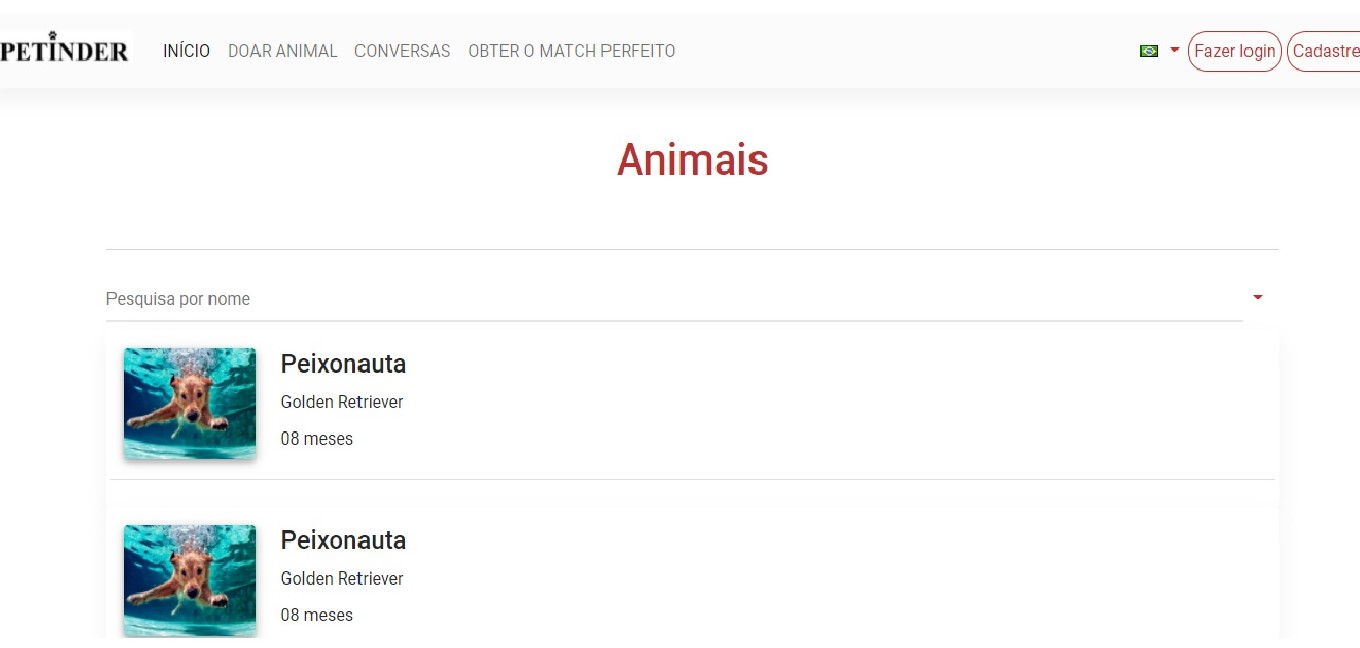
\includegraphics[scale=0.50,angle=0]{imagens/TelaInicial.jpg}
	\fonte{Elaborada pelos autores}
\end{figure}

\begin{figure}[!htbp]
    \centering
    \caption{\label{Tela Cadastro}Tela Cadastro}
	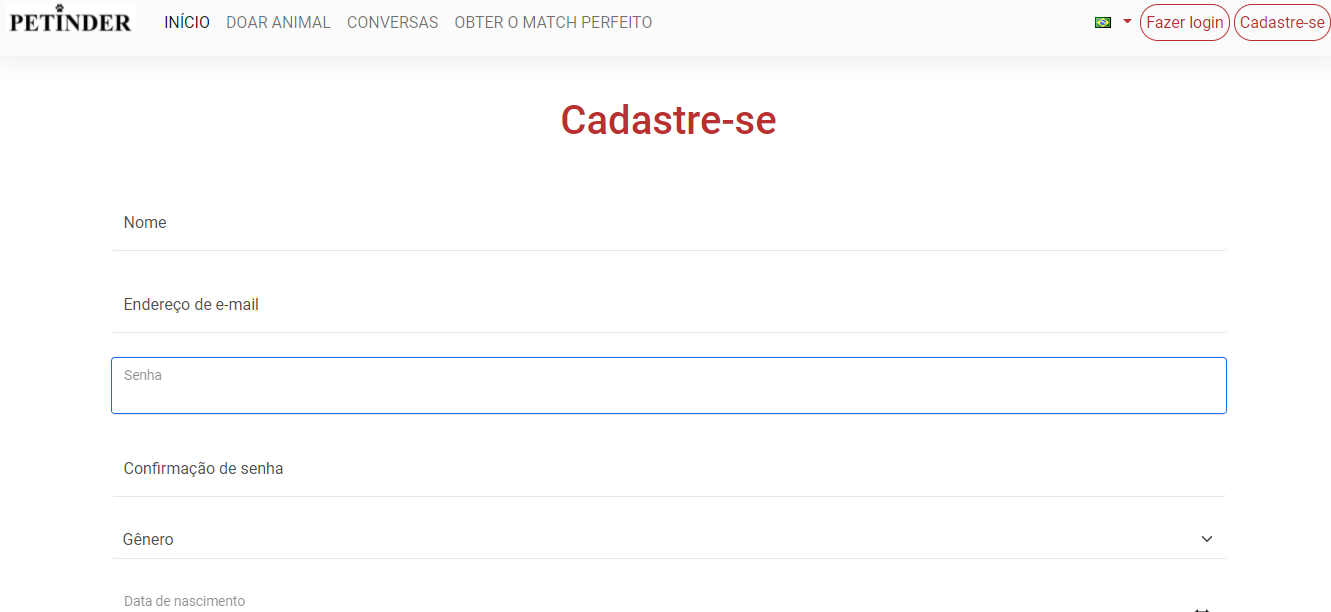
\includegraphics[scale=0.50,angle=0]{imagens/TelaCadastro.png}
	\fonte{Elaborada pelos autores}
\end{figure}

\begin{figure}[!htbp]
    \centering
    \caption{\label{Perfil Animal}Perfil Animal}
	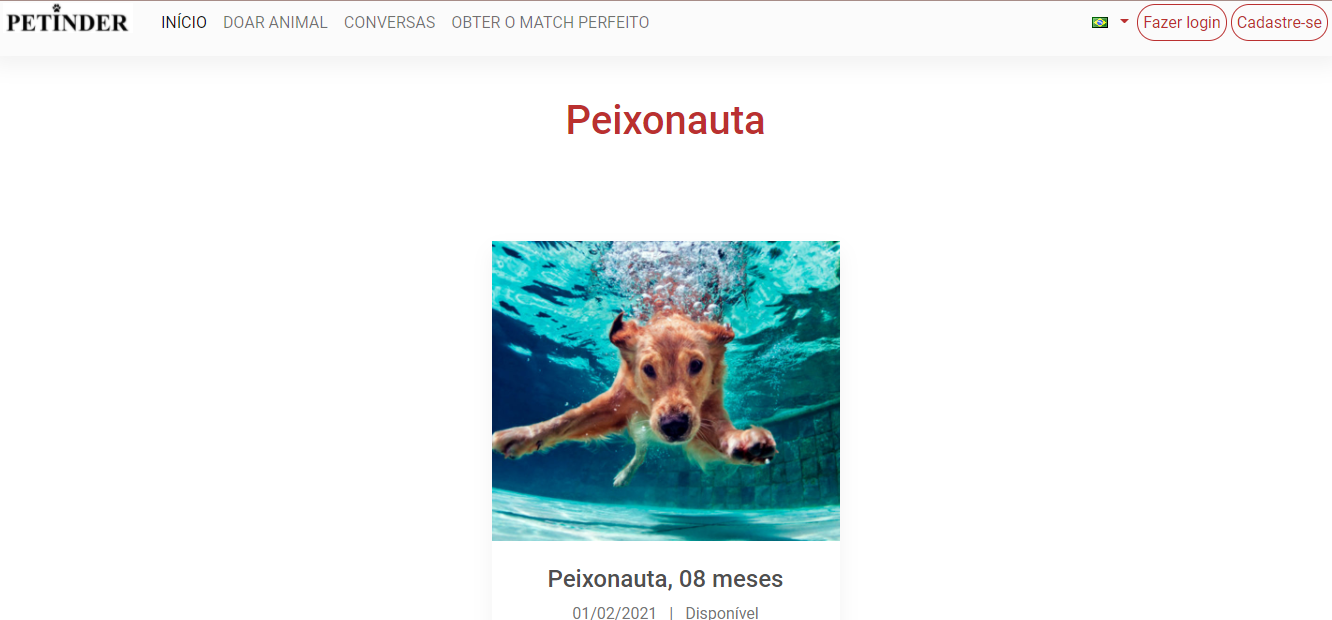
\includegraphics[scale=0.50,angle=0]{imagens/PerfilPet.png}
	\fonte{Elaborada pelos autores}
\end{figure}


\begin{figure}[!htbp]
    \centering
    \caption{\label{Tela Login}Tela Login}
	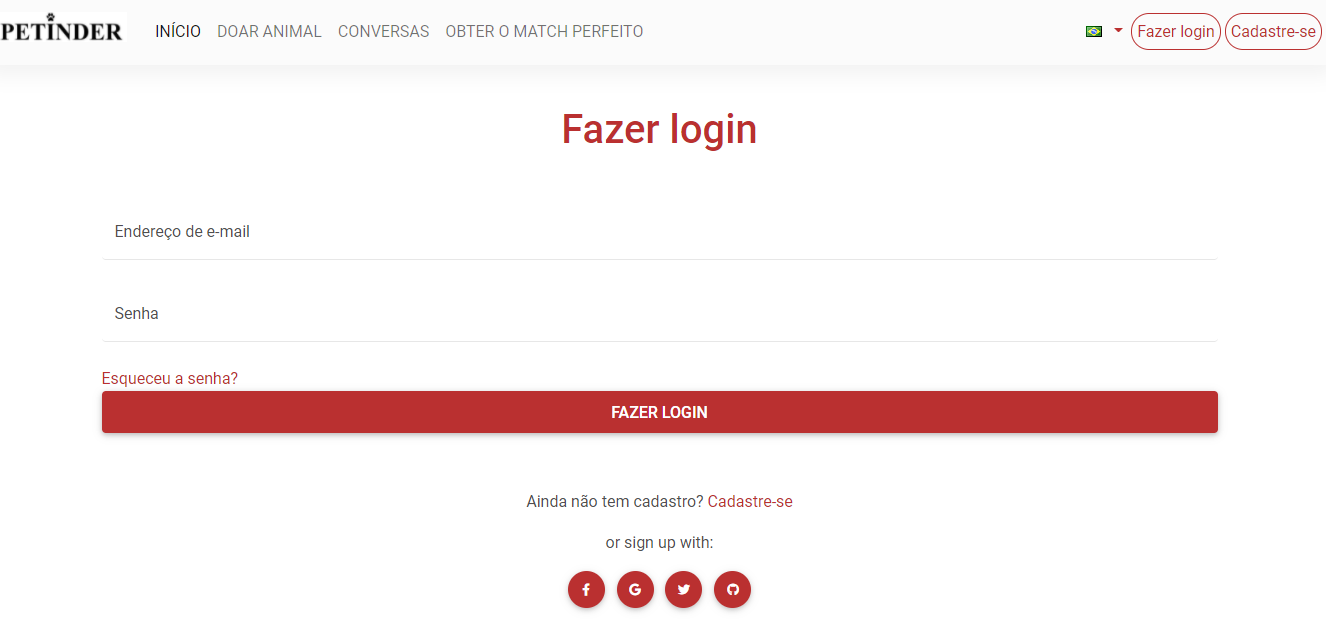
\includegraphics[scale=0.50,angle=0]{imagens/TelaLogin.png}
	\fonte{Elaborada pelos autores}
\end{figure}

\begin{figure}[!htbp]
    \centering
    \caption{\label{Cadastro Animal}Cadastro Animal}
	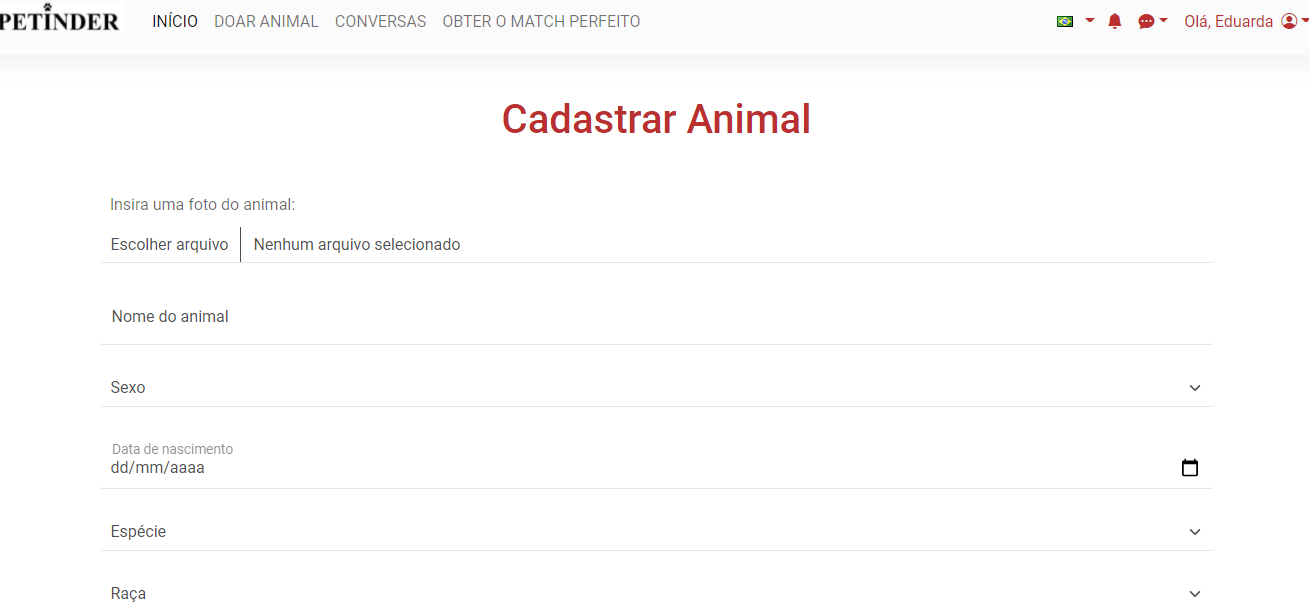
\includegraphics[scale=0.50,angle=0]{imagens/CadastroAnimal.png}
	\fonte{Elaborada pelos autores}
\end{figure}

\begin{figure}[!htbp]
    \centering
    \caption{\label{Formulario}Formulário de Adoção}
	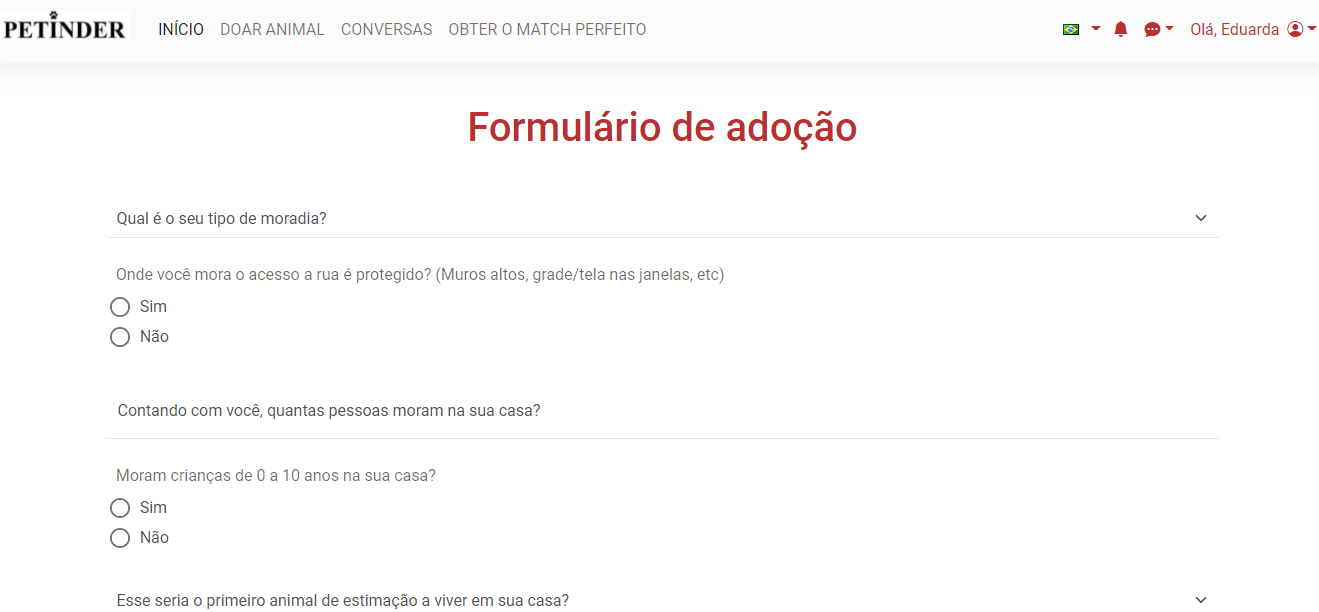
\includegraphics[scale=0.50,angle=0]{imagens/Filtros.png}
	\fonte{Elaborada pelos autores}
\end{figure}

\begin{figure}[!htbp]
    \centering
    \caption{\label{Chat}Tela de Conversas}
	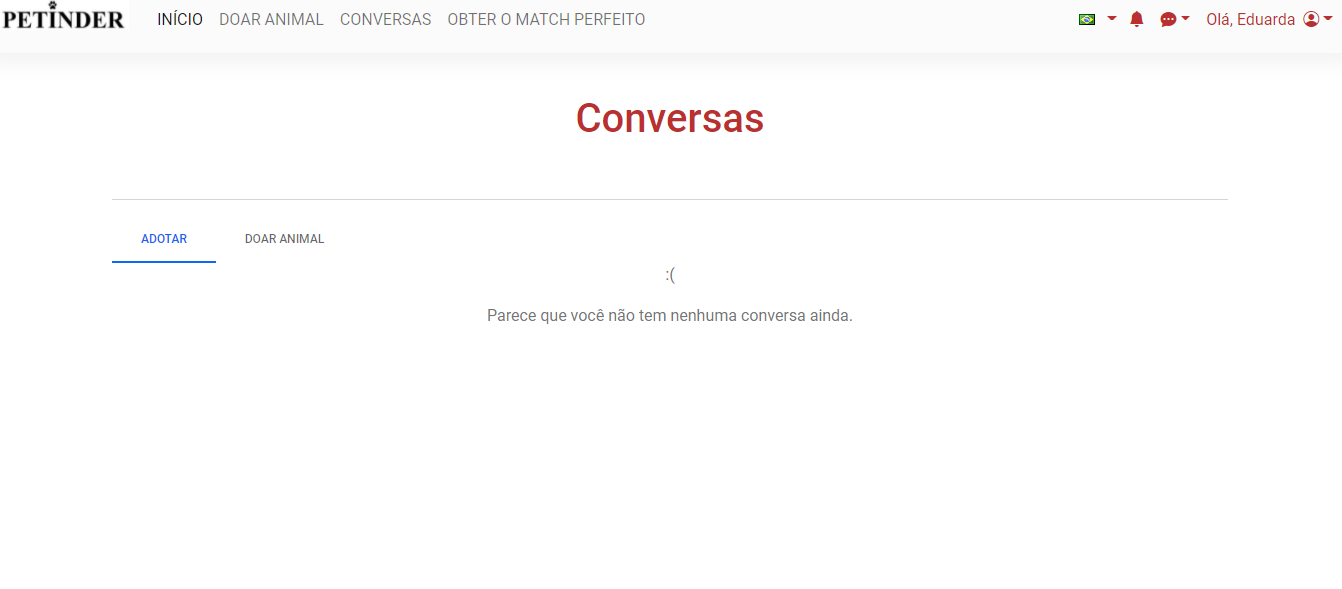
\includegraphics[scale=0.50,angle=0]{imagens/Chat.png}
	\fonte{Elaborada pelos autores}
\end{figure}

\begin{figure}[!htbp]
    \centering
    \caption{\label{Interacoes}Tela de Interações}
	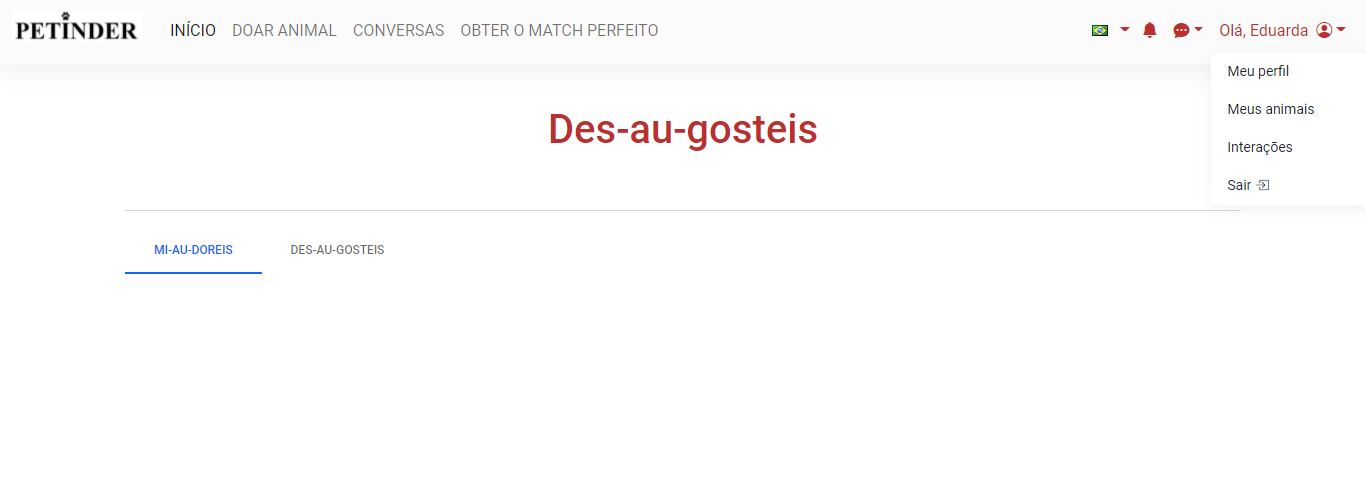
\includegraphics[scale=0.50,angle=0]{imagens/TelaInterações.png}
	\fonte{Elaborada pelos autores}
\end{figure}

\begin{figure}[!htbp]
    \centering
    \caption{\label{Perfil}Perfil Usuário}
	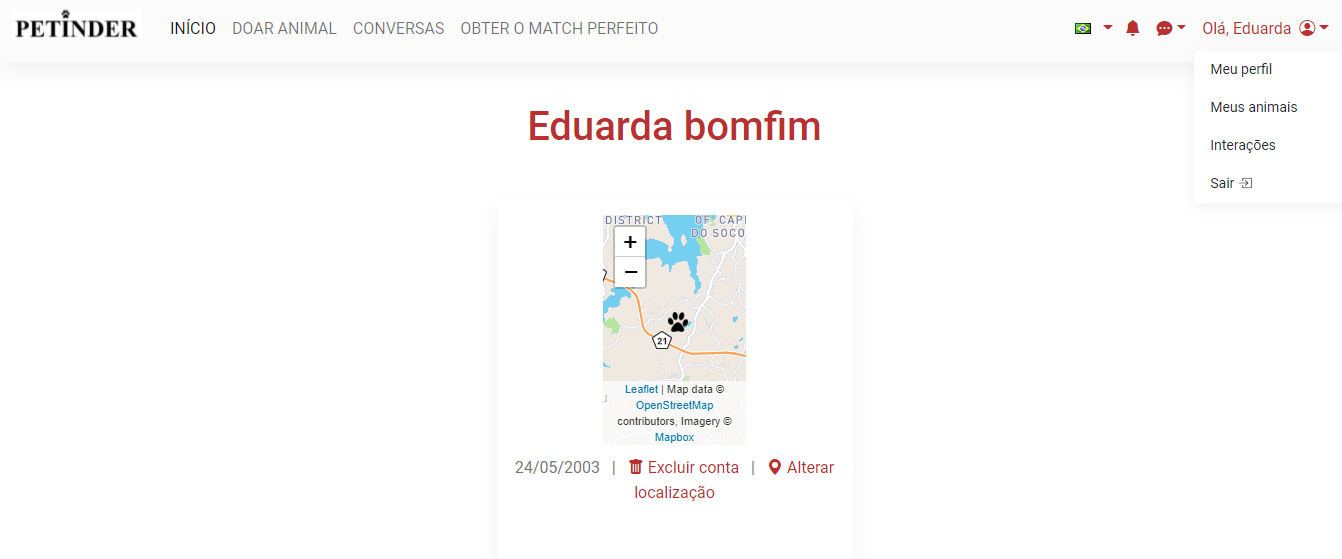
\includegraphics[scale=0.50,angle=0]{imagens/TelaPerfil.png}
	\fonte{Elaborada pelos autores}
\end{figure}

\begin{figure}[!htbp]
    \centering
    \caption{\label{Animais}Tela de Animais Cadastrados}
	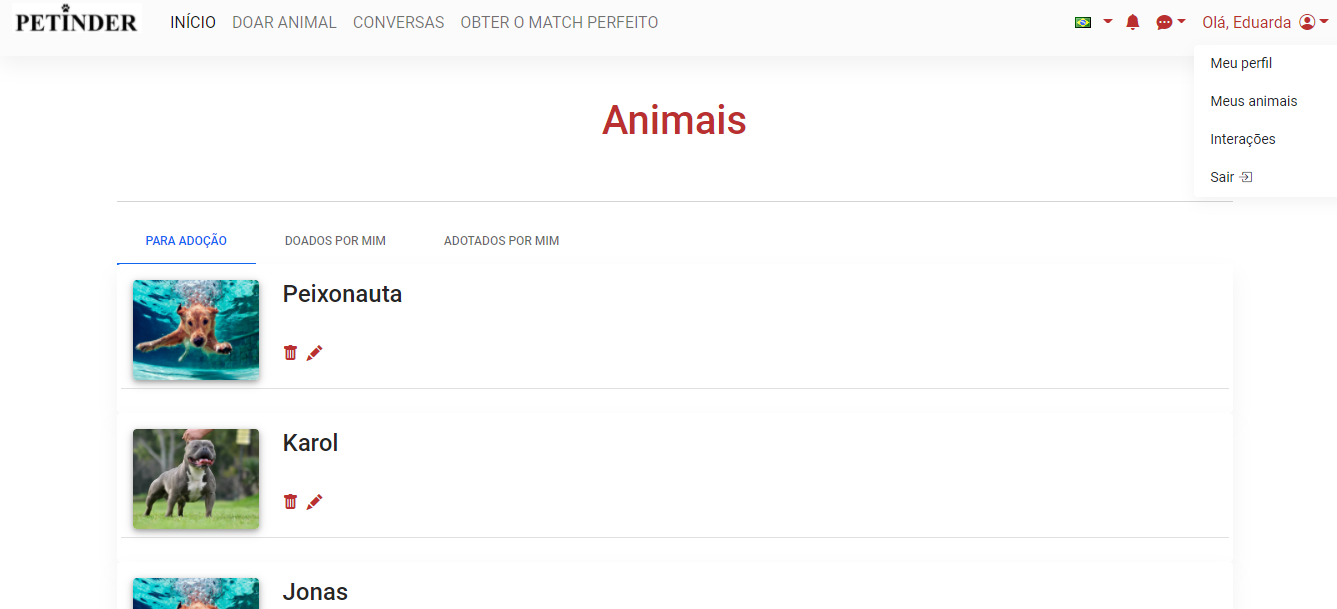
\includegraphics[scale=0.50,angle=0]{imagens/TelaAnimais.png}
	\fonte{Elaborada pelos autores}
\end{figure}

\end{flushleft}

\label{manul-usuario}

%Manual Tec
\chapter{Manual Técnico}
\label{manual-tecnico}
\begin{figure}[!htbp]
\begin{flushleft}
    \section{Modelo Entidade Relacionamento}
\end{flushleft}
    \centering
    \caption{Modelo Entidade Relacionamento}
    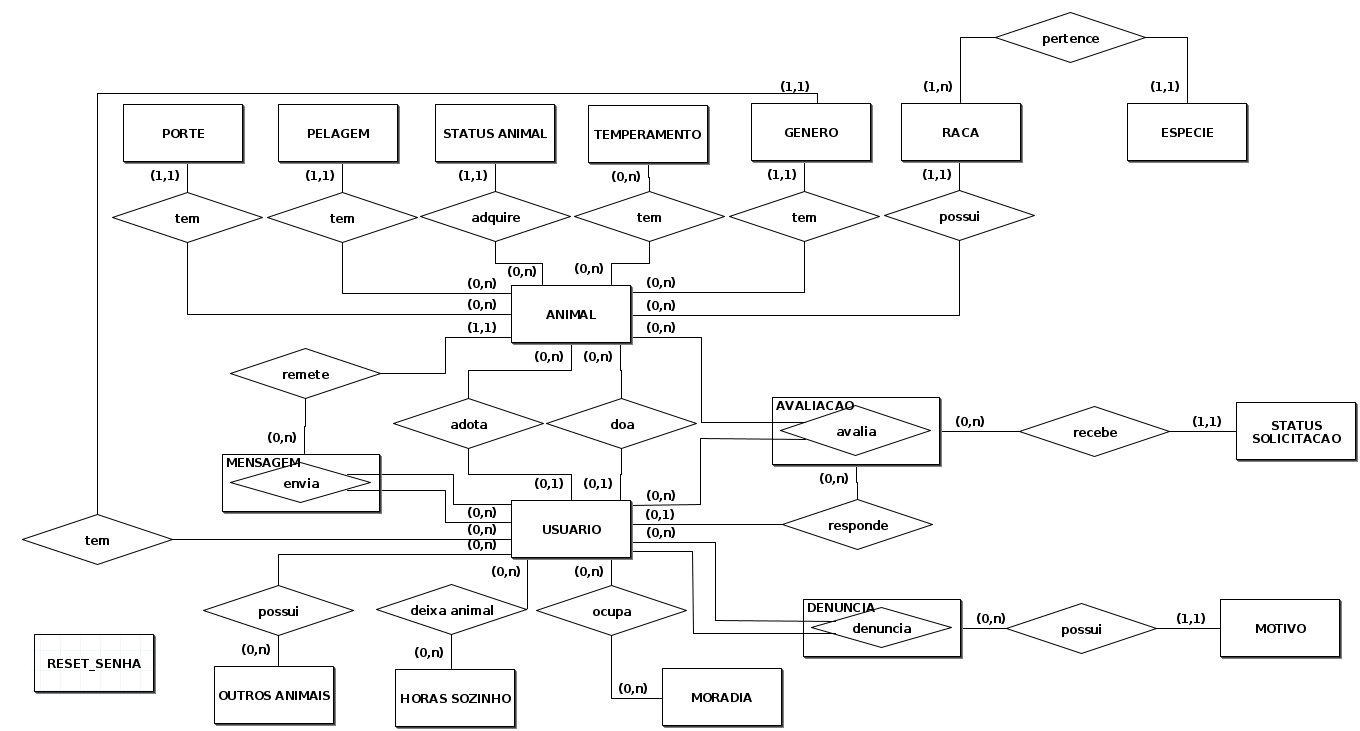
\includegraphics[scale=0.37,angle=90]{imagens/MODELOCONCEITUAL.png}
    \label{mer-tec}
    \fonte{Elaborado pelos autores}
\end{figure}

\begin{figure}[!htbp]
\begin{flushleft}
    \section{Diagrama Entidade Relacionamento}
\end{flushleft}
    \centering
    \caption{Diagrama Entidade Relacionamento}
    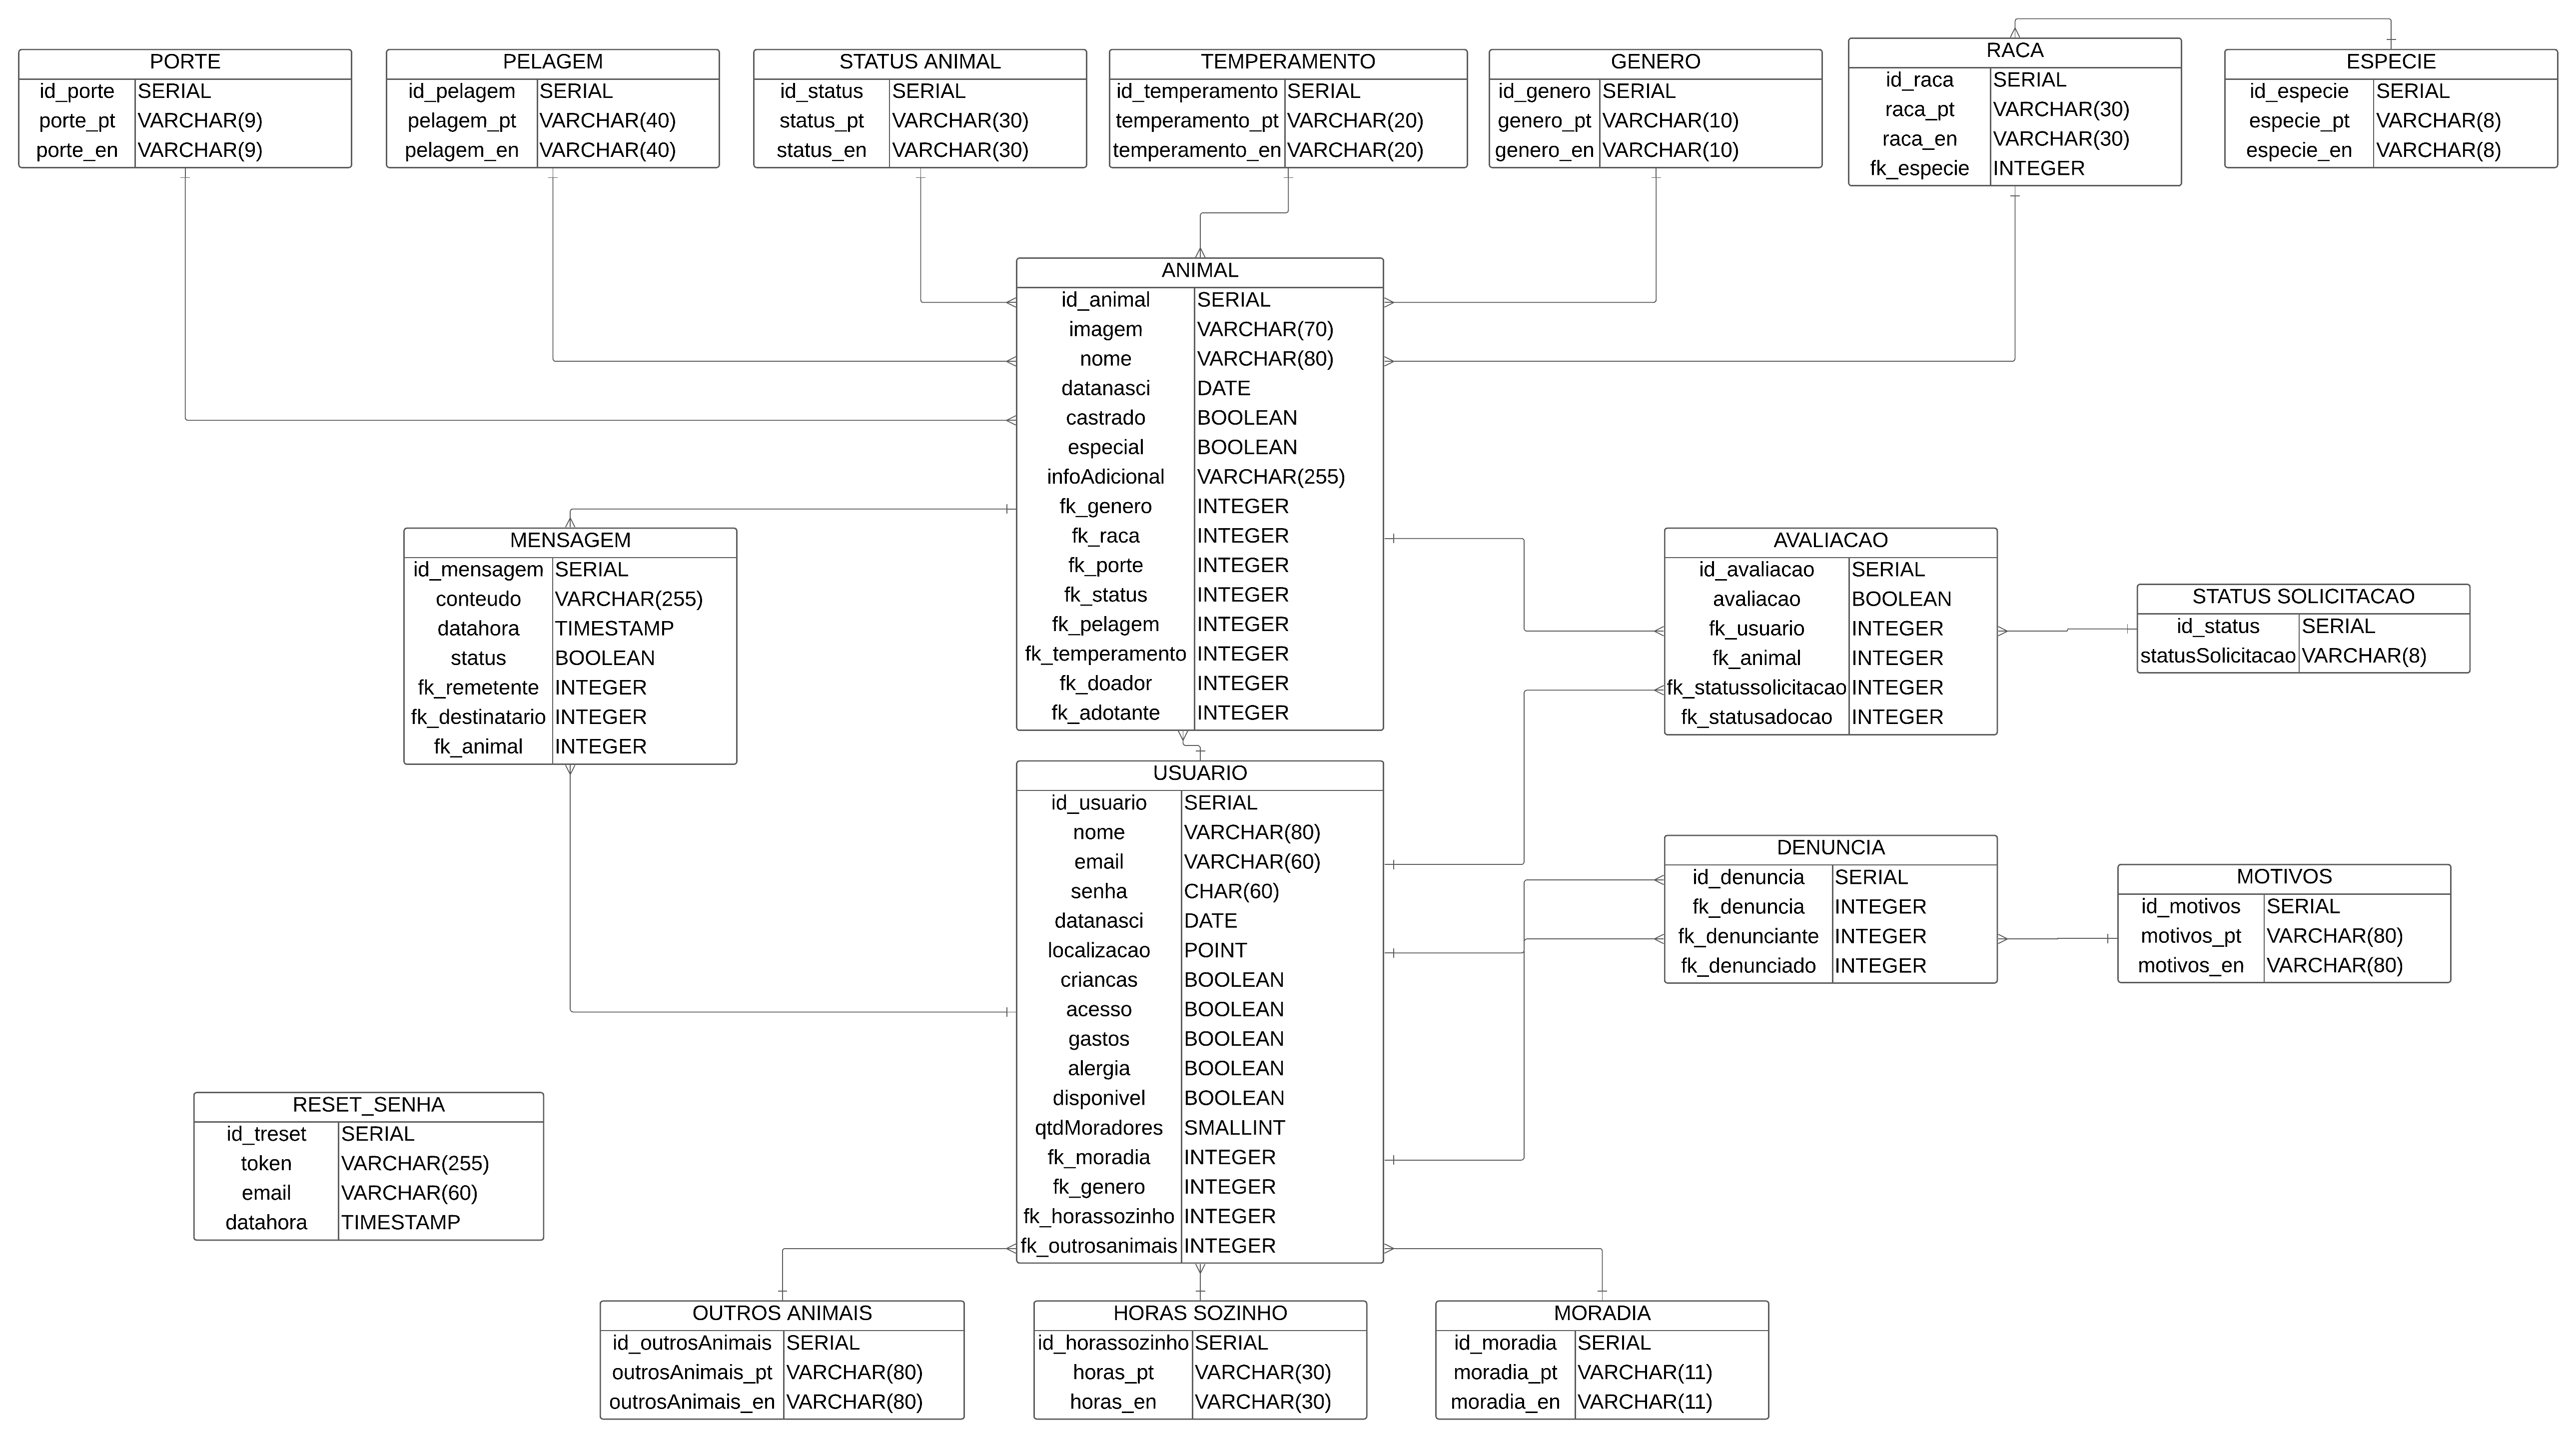
\includegraphics[scale=0.45,angle=90]{imagens/MODELOLOGICO.png}
    \label{der-tec}
    \fonte{Elaborado pelos autores}
\end{figure}

\begin{flushleft}
    \section{Dicionário de Dados}
\end{flushleft}
\begin{quadro}[!h]
\caption[Tabela Porte]{Tabela Porte}
\begin{tabular}{|c|c|p{9.1cm}|}
\hline
\multicolumn{3}{|c|}{Tabela Porte}\\ 
\hline
\thead{Atributo/Entidade} & \thead{Tipo} & \thead{Descrição}\\
\hline
Porte & Entidade & Armazenamento de porte. \\
\hline
id\_porte & Serial & Identificador do Porte. \\
\hline
porte\_pt & Varchar & Informação de porte em português. \\
\hline
porte\_en & Varchar & Informação de porte em inglês. \\
\hline
\end{tabular}
\end{quadro}

\begin{quadro}[!h]
\caption[Tabela Pelegem]{Tabela Pelagem}
\begin{tabular}{|c|c|p{9.1cm}|}
\hline
\multicolumn{3}{|c|}{Tabela Pelagem}\\
\hline
\thead{Atributo/Entidade} & \thead{Tipo} & \thead{Descrição}\\
\hline
Pelagem & Entidade & Armazenamento de informações da pelagem. \\
\hline
id\_pelagem & Serial & Identificador da pelagem. \\
\hline
pelagem\_pt & Varchar & Informação de pelagem em português. \\
\hline
pelagem\_en & Varchar & Informação de pelagem em inglês. \\
\hline
\end{tabular}
\end{quadro}

\begin{quadro}[!htbp]
\caption[Tabela Status Animal]{Tabela Status Animal}
\begin{tabular}{|c|c|c|}
\hline
\multicolumn{3}{|c|}{Tabela Status Animal}\\
\hline
\thead{Atributo/Entidade} & \thead{Tipo} & \thead{Descrição}\\
\hline
Status Animal & Entidade & Armazenamento de informações do status animal. \\
\hline
id\_status & Serial & Identificador do status animal. \\
\hline
status\_pt & Varchar & Informação do status animal em português. \\
\hline
status\_en & Varchar & Informação do status animal em inglês. \\
\hline
\end{tabular}
\end{quadro}

\begin{quadro}[!htbp]
\caption[Tabela Temperamento]{Tabela Temperamento}
\begin{tabular}{|c|c|c|}
\hline
\multicolumn{3}{|c|}{Tabela Temperamento}\\
\hline
\thead{Atributo/Entidade} & \thead{Tipo} & \thead{Descrição}\\
\hline
Temperamento & Entidade & Armazenamento de informações do temperamento. \\
\hline
id\_temperamento & Serial & Identificador do temperamento.\\
\hline
temperamento\_pt & Varchar & Informação do temperamento em português. \\
\hline
temperamento\_en & Varchar & Informação do temperamento em inglês. \\
\hline
\end{tabular}
\end{quadro}

\begin{quadro}[!htbp]
\caption[Tabela Gênero]{Tabela Gênero}
\begin{tabular}{|c|c|p{9.1cm}|}
\hline
\multicolumn{3}{|c|}{Tabela Gênero}\\
\hline
\thead{Atributo/Entidade} & \thead{Tipo} & \thead{Descrição}\\
\hline
Genero & Entidade & Armazenamento de informações do gênero. \\
\hline
id\_genero & Serial & Identificador do temperamento.\\
\hline
genero\_pt & Varchar & Informação do gênero em português. \\
\hline
genero\_en & Varchar & Informação do gênero em inglês. \\
\hline
\end{tabular}
\end{quadro}

\begin{quadro}[!htbp]
\caption[Tabela Espécie]{Tabela Espécie}
\begin{tabular}{|c|c|p{9.1cm}|}
\hline
\multicolumn{3}{|c|}{Tabela Espécie}\\
\hline
\thead{Atributo/Entidade} & \thead{Tipo} & \thead{Descrição}\\
\hline
Especie & Entidade & Armazenamento de informações da espécie. \\
\hline
id\_especie & Serial & Identificador da espécie.\\
\hline
especie\_pt & Varchar & Informação da espécie em português. \\
\hline
especie\_en & Varchar & Informação da espécie em inglês. \\
\hline
\end{tabular}
\end{quadro}

\begin{quadro}[!htbp]
\caption[Tabela Raça]{Tabela Raça}
\begin{tabular}{|c|c|p{9.1cm}|}
\hline
\multicolumn{3}{|c|}{Tabela Raça}\\
\hline
\thead{Atributo/Entidade} & \thead{Tipo} & \thead{Descrição}\\
\hline
Raca & Entidade & Armazenamento de informações da raça. \\
\hline
id\_raca & Serial & Identificador da raça.\\
\hline
raca\_pt & Varchar & Informação da raça em português. \\
\hline
raca\_en & Varchar & Informação da raça em inglês. \\
\hline
fk\_especie & Integer & Chave estrangeira de Espécie. \\
\hline
\end{tabular}
\end{quadro}

\begin{quadro}[!htbp]
\caption[Tabela Animal]{Tabela Animal}
\begin{tabular}{|c|c|p{9.1cm}|}
\hline
\multicolumn{3}{|c|}{Tabela Animal}\\
\hline
\thead{Atributo/Entidade} & \thead{Tipo} & \thead{Descrição}\\
\hline
Animal & Entidade & Armazenamento de informações do animal. \\
\hline
id\_animal & Serial & Identificador do animal. \\
\hline
imagem & Varchar & nome da imagem do animal. \\
\hline
nome & Varchar & Nome do animal. \\
\hline
datanasci & Data & Data de nascimento do animal. \\
\hline
castrado & Boolean & Se o animal é castrado, ou não. \\
\hline
especial & Boolean & Se o animal necessita tratamentos especiais. \\
\hline
infoAdicional & Varchar & Espaço para informações adicionais. \\
\hline
fk\_genero & Integer & Chave estrangeira de Gênero. \\
\hline
fk\_raca & Integer & Chave estrangeira de Raça. \\
\hline
fk\_porte & Integer & Chave estrangeira de Porte. \\
\hline
fk\_status & Integer & Chave estrangeira de Status Animal. \\
\hline
fk\_pelagem & Integer & Chave estrangeira de Pelagem. \\
\hline
fk\_temperamento & Integer & Chave estrangeira de Temperamento. \\
\hline
fk\_doador & Integer & Chave estrangeira de Doador. \\
\hline
fk\_adotante & Integer & Chave estrangeira de Adotante.\\
\hline
\end{tabular}
\end{quadro}

\begin{quadro}[!htbp]
\caption[Tabela Mensagem]{Tabela Mensagem}
\begin{tabular}{|c|c|p{8.8cm}|}
\hline
\multicolumn{3}{|c|}{Tabela Mensagem}\\
\hline
\thead{Atributo/Entidade} & \thead{Tipo} & \thead{Descrição}\\
\hline
Mensagem & Entidade & Armazenamento de mensagens. \\
\hline
id\_mensagem & Serial & Identificador de mensagens. \\
\hline
conteudo & Varchar & Conteúdo da mensagem. \\
\hline
datahora & Timestamp & Data e hora de envio das mensagens. \\
\hline
status & Boolean & Mensagem lida ou não lida. \\
\hline
fk\_remetente & Integer & Chave estrangeira de Remetente. \\
\hline
fk\_destinatario & Integer & Chave estrangeira de Destinatário. \\
\hline
fk\_animal & Integer & Chave estrangeira de Animal. \\
\hline
\end{tabular}
\end{quadro}

\begin{quadro}[!htbp]
\caption[Tabela Status Solicitação]{Tabela Status Solicitação}
\begin{tabular}{|c|c|p{9.1cm}|}
\hline
\multicolumn{3}{|c|}{Tabela Status Solicitação}\\
\hline
\thead{Atributo/Entidade} & \thead{Tipo} & \thead{Descrição}\\
\hline
Status Solicitação & Entidade & Armazenamento de Status de Solicitação. \\
\hline
id\_status & Serial & Identificador do Status Solicitação. \\
\hline
statusSolicitacao & Varchar & Estado da solicitação. \\
\hline
\end{tabular}
\end{quadro}

\begin{quadro}[!htbp]
\caption[Tabela Avaliação]{Tabela Avaliação}
\begin{tabular}{|c|c|p{9.1cm}|}
\hline
\multicolumn{3}{|c|}{Tabela Avaliação}\\
\hline
\thead{Atributo/Entidade} & \thead{Tipo} & \thead{Descrição}\\
\hline
Avaliacao & Entidade & Armazenamento de informações da avaliação. \\
\hline
id\_avaliacao & Serial & Identificador de avaliação. \\
\hline
avaliacao & Boolean &  Detalhamento da avaliação. \\
\hline
fk\_usuario & Integer & Chave estrangeira de Usuário. \\
\hline
fk\_animal & Integer & Chave estrangeira de Animal. \\
\hline
fk\_statussolicitacao & Integer & Chave estrangeira de Status Solicitação. \\
\hline
fk\_statusadocao & Integer & Chave estrangeira de Status Adoção. \\
\hline
\end{tabular}
\end{quadro}

\begin{quadro}[!htbp]
\caption[Tabela Motivos]{Tabela Motivos}
\begin{tabular}{|c|c|p{9.1cm}|}
\hline
\multicolumn{3}{|c|}{Tabela Motivos}\\
\hline
\thead{Atributo/Entidade} & \thead{Tipo} & \thead{Descrição}\\
\hline
Motivos & Entidade & Armazenamento de informações do motivo. \\
\hline
id\_motivos & Serial & Identificador de motivos.\\
\hline
motivos\_pt & Varchar & Motivos, em português. \\
\hline 
motivos\_en & Varchar & Motivos, em inglês. \\
\hline
\end{tabular}
\end{quadro}

\begin{quadro}[!htbp]
\caption[Tabela Denúncia]{Tabela Denúncia}
\begin{tabular}{|c|c|p{9.1cm}|}
\hline
\multicolumn{3}{|c|}{Tabela Denúncia}\\
\hline
\thead{Atributo/Entidade} & \thead{Tipo} & \thead{Descrição}\\
\hline
Denuncia & Entidade & Armazenamento de informações de denúncias. \\
\hline
id\_denuncia & Serial & Identificador de denuncia. \\
\hline
fk\_denuncia & Integer & Chave estrangeira de Denuncia. \\
\hline
fk\_denunciante & Integer & Chave estrangeira de Denunciante. \\
\hline
fk\_denunciado & Integer & Chave estrangeira de Denunciado. \\
\hline
\end{tabular}
\end{quadro}

\begin{quadro}[!htbp]
\caption[Tabela Outros Animais]{Tabela Outros Animais}
\begin{tabular}{|c|c|p{9.1cm}|}
\hline
\multicolumn{3}{|c|}{Tabela Outros Animais}\\
\hline
\thead{Atributo/Entidade} & \thead{Tipo} & \thead{Descrição}\\
\hline
Outros Animais & Entidade & Armazenamento de informações do outros animais. \\
\hline
id\_outrosAnimais & Serial & Identificador de outros animais.\\
\hline
outrosAnimais\_pt & Varchar & Informações de outros animais em português. \\
\hline 
outrosAnimais\_en & Varchar & Informações de outros animais em inglês. \\
\hline
\end{tabular}
\end{quadro}

\begin{quadro}[!htbp]
\caption[Tabela Horas Sozinho]{Tabela Horas Sozinho}
\begin{tabular}{|c|c|p{9.1cm}|}
\hline
\multicolumn{3}{|c|}{Tabela Horas Sozinho}\\
\hline
\thead{Atributo/Entidade} & \thead{Tipo} & \thead{Descrição}\\
\hline
Horas Sozinho & Entidade & Armazenamento de informações do horas sozinho. \\
\hline
id\_horassozinho & Serial & Identificador de horas sozinho.\\
\hline
horas\_pt & Varchar & Informações de horas sozinho em português. \\
\hline 
horas\_en & Varchar & Informações de horas sozinho em inglês. \\
\hline
\end{tabular}
\end{quadro}

\begin{quadro}[!htbp]
\caption[Tabela Moradia]{Tabela Moradia}
\begin{tabular}{|c|c|p{9.1cm}|}
\hline
\multicolumn{3}{|c|}{Tabela Moradia}\\
\hline
\thead{Atributo/Entidade} & \thead{Tipo} & \thead{Descrição}\\
\hline
Moradia & Entidade & Armazenamento de informações de moradia. \\
\hline
id\_moradia & Serial & Identificador de moradia. \\
\hline
moradia\_pt & Varchar & Informações de moradia em português. \\
\hline 
moradia\_en & Varchar & Informações de moradia em inglês. \\
\hline
\end{tabular}
\end{quadro}

\begin{quadro}[!ht]
\caption[Tabela Usuário]{Tabela Usuário}
\begin{tabular}{|c|c|p{9.1cm}|}
\hline
\multicolumn{3}{|c|}{Tabela Usuário}\\ 
\hline
\thead{Atributo/Entidade} & \thead{Tipo} & \thead{Descrição}\\
\hline
Usuario & Entidade &  Armazenamento de informações do usuário. \\
\hline
id\_usuario & Serial &  Identificador do usuário. \\
\hline
nome & Varchar & Nome do usuário \\
\hline
email & Varchar & Endereço eletrôncio do usuário. \\
\hline
senha & Char & Senha de acesso do usuário. \\
\hline
datanasci & Date & Data de Nascimento do usuário. \\
\hline
localizacao & Point & Local do usuário. \\
\hline
criancas & Boolean & Se há ou não há crianças na residência do usuário. \\
\hline
acesso & Boolean & Se a rua é de fácil acesso. \\
\hline
gastos & Boolean & Se os gasto já estão previstos no orçamento. \\
\hline
alergia & Boolean & Se há alguém na residência com alergia. \\
\hline
disponivel & Boolean & Retorna "falso" quando sua é banida por ser denunciado três vezes. \\
\hline
qntMoradores & SmallInt & Quantos moradores há na residência. \\
\hline
fk\_moradia & Interger & Chave estrangeira de Moradia. \\ 
\hline
fk\_genero & Interger & Chave estrangeira de Gênero. \\ 
\hline
fk\_horassozinho & Interger & Chave estrangeira de Horas Sozinho. \\ 
\hline
fk\_outrosanimais & Interger & Chave estrangeira de Outros Animais. \\ 
\hline
\end{tabular}
\fonte{Elaborado pelos autores}
\end{quadro}

\begin{quadro}[!ht]
\caption[Tabela Reset Senha]{Tabela Reset Senha}
\begin{tabular}{|c|c|p{9.1cm}|}
\hline
\multicolumn{3}{|c|}{Tabela Reset Senha}\\ 
\hline
\thead{Atributo/Entidade} & \thead{Tipo} & \thead{Descrição}\\
\hline
Reset_senha & Entidade & Armazenamento de informações de reset senha. \\
\hline
id_reset & Serial & Identificador de reset senha. \\
\hline
token & Varchar & Enviado no \gls{E-mail} junto com o \textit{link} para confirmação. \\
\hline
email & Varchar & Endereço eletrônico do usuário. \\
\hline
datahora & Timestamp & Data e hora que foi requisitado o reset de senha. \\
\hline
\end{tabular}
\end{quadro}

\newpage
\begin{figure}[!htbp]
\begin{flushleft}
    \section{Diagrama Caso de Uso}
\end{flushleft}
    \centering
    \caption{Diagrama Casos de Uso}
    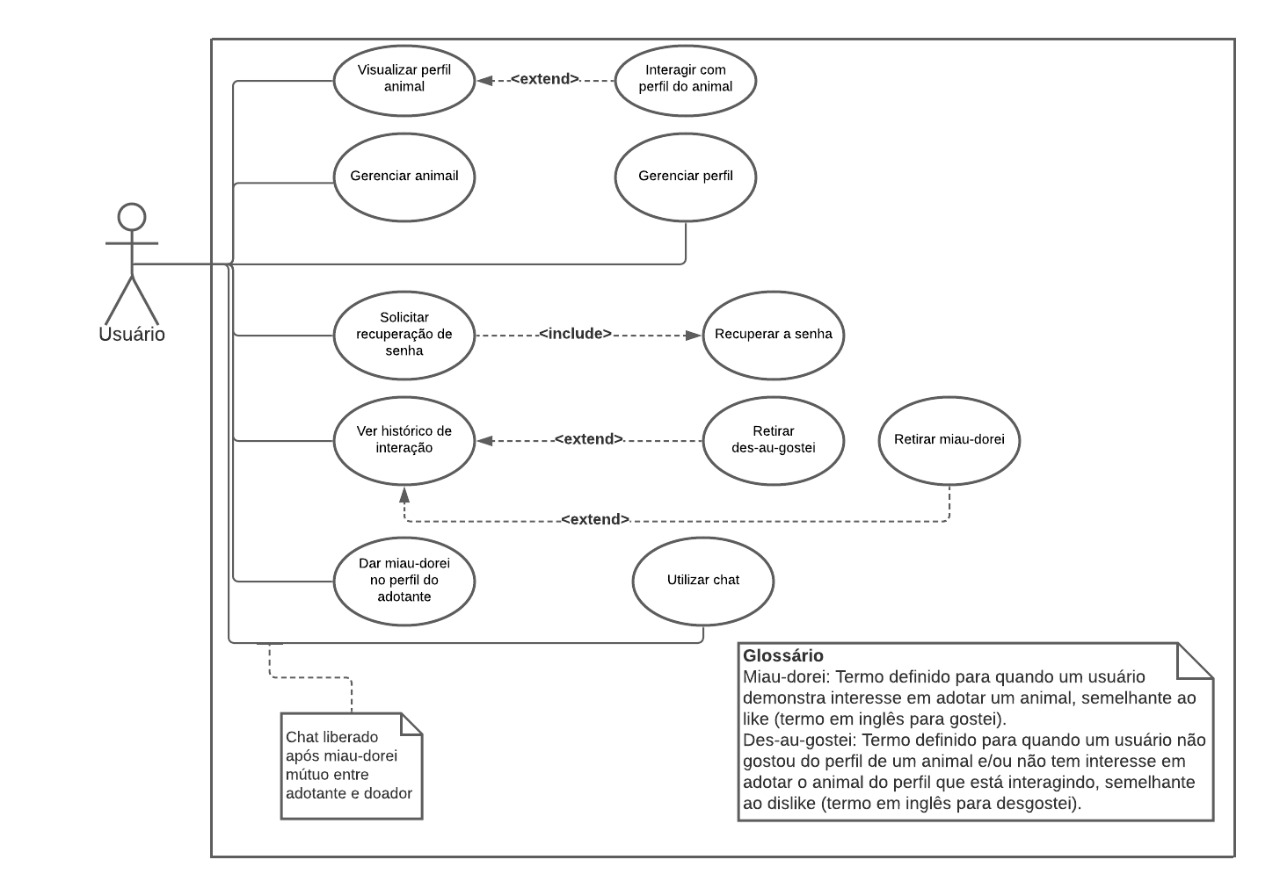
\includegraphics[scale=0.45,angle=90,pagecommand=\chapter{Diagrama Casos de Uso}]{imagens/CasosDeUsoPETINDER.jpeg}
    \label{diagrama-casos}
    \fonte{Elaborado pelos autores}
\end{figure}


%--------------CASOS-DE-USO--------------
\begin{quadro}[!h]
\centering
\caption[Casos de Uso]{Casos de Uso (UC)}
\begin{tabular}{|p{0.7cm}|p{5.55cm}|p{7.7cm}|}
\hline
\thead{UC} & \thead{Nome} & \thead{Descrição}\\
\hline
01 & Visualizar perfil do animal &  Acesso ao perfil de um animal, sem ser necessário o cadastro. \\ 
\hline
02 & Interagir com perfil do animal &  Dar \gls{Miau-dorei} ou \gls{Des-au-gostei} no perfil de um animal. \\ 
\hline
03 & Gerenciar animal &  Usuário responsável por alterações no perfil do animal. \\ 
\hline
04 & Gerenciar perfil & Usuário fazer alterações no seu perfil. \\ 
\hline
05 & Solicitar recuperação de senha & Solicitação do usuário para envio de \gls{E-mail} para ação de recuperar senha. \\
\hline
06 & Recuperar senha & Criação de nova senha. \\
\hline
07 & Ver histórico de interação & Acesso a uma lista de interações feitas. \\
\hline
08 & Retirar \gls{Des-au-gostei} & Desfazer a interação de desgostar no perfil de um usuário ou animal. \\
\hline
09 & Retiar \gls{Miau-dorei} & Desfazer a interação de gostar no perfil de um usuário ou animal. \\
\hline
10 & Dar \gls{Miau-dorei} no perfil do adotante & Interação feita pelo doador de gostar no perfil do adotante. \\
\hline
11 & Utilizar \textit{chat} & Disposto apenas quando há o \gls{Match} entre adotante e doador. Utilizado para conversa e troca de informações. \\
\hline
\end{tabular}
\fonte{Elaborado pelos autores}
\end{quadro}

%--------------ATORES--------------
\begin{quadro}[!h]
\caption[Caso de Uso - Atores]{Caso de Uso - Atores}
\begin{tabular}{|c|c|p{12.1cm}|}
\hline
\thead{Ator} & \thead{Nome} & \thead{Descrição}\\
\hline
01 & Usuário &  Pessoa que faça uso do site, podendo ou não ser cadastrado. \\
\hline
\end{tabular}
\fonte{Elaborado pelos autores}
\end{quadro}

%--------------UC-1--------------
\begin{quadro}[!htbp]
\caption[Detalhamento 1$^\circ$ Caso de Uso]{Detalhamento 1$^\circ$ Caso de Uso}
\begin{tabular}{|p{4cm}|p{9.95cm}|}
\hline
\multicolumn{2}{|c|}{Detalhamento do 1$^\circ$ Caso de Uso}\\ 
\hline
Nome & Visualizar perfil do animal \\
\hline
Objetivo & O acesso à informações do animal.  \\
\hline
Atores & Usuário. \\
\hline
Grau de Importância & Alto. \\
\hline
Frequência de Uso & Alta. \\
\hline
Pré-Condição & Acessar o \textit{link} da página \textit{web}. \\
\hline
Pós-Condição & Cadastrar-se ou logar-se. No caso de já estar logado, o usuário pode interagir com o perfil do animal. \\
\hline
Fluxo Principal & 1)Escolher um animal na página inicial; 2) Abrir o perfil do animal escolhido.\\
\hline
Fluxo Alternativo & -\\
\hline
\end{tabular}
\fonte{Elaborado pelos autores}
\end{quadro}

%--------------UC-2--------------
\begin{quadro}[!htbp]
\caption[Detalhamento 2$^\circ$ Caso de Uso]{Detalhamento 2$^\circ$ Caso de Uso}
\begin{tabular}{|p{4cm}|p{9.95cm}|}
\hline
\multicolumn{2}{|c|}{Detalhamento do 2$^\circ$ Caso de Uso}\\ 
\hline
Nome & Interagir com perfil do animal  \\
\hline
Objetivo & Dar \gls{Miau-dorei} ou \gls{Des-au-gostei} o perfil do animal. \\
\hline
Atores & Usuário. \\
\hline
Grau de Importância & Alto. \\
\hline
Frequência de Uso & Alta. \\
\hline
Pré-Condição & Estar logado e estar na página do perfil do animal. \\
\hline
Pós-Condição & Acessar histórico de interação ou interação do doador com o perfil do adotante. \\
\hline
Fluxo Principal & 1) Fazer cadastro ou \textit{login};; 2) Acessar o perfil do animal; 3) Dar \gls{Miau-dorei} ou \gls{Des-au-gostei} no perfil. \\
\hline
Fluxo Alternativo & 1) Não é necessário realizar o passo 1 caso o usuário já esteja logado.\\
\hline
\end{tabular}
\fonte{Elaborado pelos autores}
\end{quadro}

%--------------UC-3--------------
\begin{quadro}[!htbp]
\caption[Detalhamento 3$^\circ$ Caso de Uso]{Detalhamento 3$^\circ$ Caso de Uso}
\begin{tabular}{|p{4cm}|p{9.95cm}|}
\hline
\multicolumn{2}{|c|}{Detalhamento do 3$^\circ$ Caso de Uso}\\ 
\hline
Nome & Gerenciar animal \\
\hline
Objetivo & Usuário responsável possa fazer alterações no perfil do animal. \\
\hline
Atores & Usuário. \\
\hline
Grau de Importância & Alto. \\
\hline
Frequência de Uso & Alta. \\
\hline
Pré-Condição & Ser um usuário cadastrado e ter um animal cadastrado. \\
\hline
Pós-Condição & No caso de mais de um animal cadastrado, o usuário responsável escolherá o perfil que será gerenciado; e edições das informações. \\
\hline
Fluxo Principal & 1) Acessar o perfil; 3) Acessar o perfil do animal que será gerenciado; 4) Fazer as alterações; 5) Salvar as alterações. \\
\hline
Fluxo Alternativo & 1) Em caso de erro, refazer as alterações \\
\hline
\end{tabular}
\fonte{Elaborado pelos autores}
\end{quadro}

%--------------UC-4--------------
\begin{quadro}[!htbp]
\caption[Detalhamento 4$^\circ$ Caso de Uso]{Detalhamento 4$^\circ$ Caso de Uso}
\begin{tabular}{|p{4cm}|p{9.95cm}|}
\hline
\multicolumn{2}{|c|}{Detalhamento do 4$^\circ$ Caso de Uso}\\ 
\hline
Nome & Gerenciar perfil \\
\hline
Objetivo & Usuário fazer alterações em seu perfil. \\
\hline
Atores & Usuário. \\
\hline
Grau de Importância & Alto. \\
\hline
Frequência de Uso & Alta. \\
\hline
Pré-Condição & Estar logado. \\
\hline
Pós-Condição & Visualizar, doar ou adotar.  \\
\hline
Fluxo Principal & 1)Acessar o perfil; 2) Editar; 3) Salvar alterações. \\
\hline
Fluxo Alternativo & 1) Em caso de erro, refazer a edição. \\
\hline
\end{tabular}
\fonte{Elaborado pelos autores}
\end{quadro}

%--------------UC-5--------------
\begin{quadro}[!htbp]
\caption[Detalhamento 5$^\circ$ Caso de Uso]{Detalhamento 5$^\circ$ Caso de Uso}
\begin{tabular}{|p{4cm}|p{9.95cm}|}
\hline
\multicolumn{2}{|c|}{Detalhamento do 5$^\circ$ Caso de Uso}\\ 
\hline
Nome & Solicitar recuperação de senha \\
\hline
Objetivo & Iniciar o pedido de recuperação de senha. \\
\hline
Atores & Usuário. \\
\hline
Grau de Importância & Alto. \\
\hline
Frequência de Uso & Média. \\
\hline
Pré-Condição & Ter cadastro. \\
\hline
Pós-Condição & Fazer a alteração por meio do \gls{E-mail} enviado ao que foi cadastrado. \\
\hline
Fluxo Principal & 1) Iniciar o pedido de recuperação de senha; 2) Verificar se o \gls{E-mail} cadastrado está certo; 3 Verificar a caixa de entrada.\\
\hline
Fluxo Alternativo & 1) Se o \gls{E-mail} cadastrado não estiver certo, o usuário deve fazer a alteração; 2) Caso o \gls{E-mail} não esteja na caixa de entrada, o usuário deve verificar o spam. \\
\hline
\end{tabular}
\fonte{Elaborado pelos autores}
\end{quadro}

%--------------UC-6--------------
\begin{quadro}[!htbp]
\caption[Detalhamento 6$^\circ$ Caso de Uso]{Detalhamento 6$^\circ$ Caso de Uso}
\begin{tabular}{|p{4cm}|p{9.95cm}|}
\hline
\multicolumn{2}{|c|}{Detalhamento do 6$^\circ$ Caso de Uso}\\ 
\hline
Nome & Recuperar senha \\
\hline
Objetivo & Criação de nova senha. \\
\hline
Atores & Usuário. \\
\hline
Grau de Importância & Alto. \\
\hline
Frequência de Uso & Média. \\
\hline
Pré-Condição & Ter feito a solicitação de recuperação de senha e ter aberto o \textit{link} enviado. \\
\hline
Pós-Condição & Fazer e salvar a nova senha, e \textit{login}.\\
\hline
Fluxo Principal & 1) Abrir \textit{link} enviado ao \gls{E-mail}; 2) Inserir a nova senha e a confirmação; 3) Salvar as alterações. \\
\hline
Fluxo Alternativo & - \\
\hline
\end{tabular}
\fonte{Elaborado pelos autores}
\end{quadro}

%--------------UC-7--------------
\begin{quadro}[!htbp]
\caption[Detalhamento 7$^\circ$ Caso de Uso]{Detalhamento 7$^\circ$ Caso de Uso}
\begin{tabular}{|p{4cm}|p{9.95cm}|}
\hline
\multicolumn{2}{|c|}{Detalhamento do 7$^\circ$ Caso de Uso}\\ 
\hline
Nome & Ver histórico de interação \\
\hline
Objetivo & Acesso a lista de interações. \\
\hline
Atores & Usuário. \\
\hline
Grau de Importância & Médio.\\
\hline
Frequência de Uso & Média. \\
\hline
Pré-Condição & Estar logado, e já ter interagido com algum perfil. \\
\hline
Pós-Condição & Acesso as interações. \\
\hline
Fluxo Principal & 1) Acessar o perfil; 2) Clicar em "Histórico de interação"; \\
\hline
Fluxo Alternativo & - \\
\hline
\end{tabular}
\fonte{Elaborado pelos autores}
\end{quadro}

%--------------UC-8--------------
\begin{quadro}[!htbp]
\caption[Detalhamento 8$^\circ$ Caso de Uso]{Detalhamento 8$^\circ$ Caso de Uso}
\begin{tabular}{|p{4cm}|p{9.95cm}|}
\hline
\multicolumn{2}{|c|}{Detalhamento do 8$^\circ$ Caso de Uso}\\ 
\hline
Nome & Retirar \gls{Des-au-gostei} \\
\hline
Objetivo & Desfazer a interação de \gls{Des-au-gostei} do perfil de um usuário ou animal. \\
\hline
Atores & Usuário. \\
\hline
Grau de Importância & Alto. \\
\hline
Frequência de Uso & Média. \\
\hline
Pré-Condição & Já ter dado \gls{Des-au-gostei}. \\
\hline
Pós-Condição & Poder trocar a interação, ou não fazer outra interação. \\
\hline
Fluxo Principal & 1) Acessar o histórico de interação; 2) Abrir o perfil do animal ou usuário; 3) Retirar a interação. \\
\hline
Fluxo Alternativo & 1) Acessar direto o perfil do animal ou usuário. \\
\hline
\end{tabular}
\fonte{Elaborado pelos autores}
\end{quadro}

%--------------UC-9--------------
\begin{quadro}[!htbp]
\caption[Detalhamento 9$^\circ$ Caso de Uso]{Detalhamento 9$^\circ$ Caso de Uso}
\begin{tabular}{|p{4cm}|p{9.95cm}|}
\hline
\multicolumn{2}{|c|}{Detalhamento do 9$^\circ$ Caso de Uso}\\ 
\hline
Nome & Retirar \gls{Miau-dorei} \\
\hline
Objetivo & Desfazer a interação de \gls{Miau-dorei} do perfil de um usuário ou animal. \\
\hline
Atores & Usuário. \\
\hline
Grau de Importância & Alto. \\
\hline
Frequência de Uso & Média. \\
\hline
Pré-Condição & Já ter dado \gls{Miau-dorei}. \\
\hline
Pós-Condição & Poder trocar a interação, ou não fazer outra interação. \\
\hline
Fluxo Principal & 1) Acessar o histórico de interação; 2) Abrir o perfil do animal ou usuário; 3) Retirar a interação. \\
\hline
Fluxo Alternativo & 1) Acessar direto o perfil do animal ou usuário. \\
\hline
\end{tabular}
\fonte{Elaborado pelos autores}
\end{quadro}

%--------------UC-10--------------
\begin{quadro}[!htbp]
\caption[Detalhamento 10$^\circ$ Caso de Uso]{Detalhamento 10$^\circ$ Caso de Uso}
\begin{tabular}{|p{4cm}|p{9.95cm}|}
\hline
\multicolumn{2}{|c|}{Detalhamento do 10$^\circ$ Caso de Uso}\\ 
\hline
Nome & Dar \gls{Miau-dorei} no perfil do adotante. \\
\hline
Objetivo & Interação de gostar do doador no perfil do adotante.\\
\hline
Atores & Usuário. \\
\hline
Grau de Importância & Alto. \\
\hline
Frequência de Uso & Alta. \\
\hline
Pré-Condição & O adotante ter dado \gls{Miau-dorei} no perfil de algum animal cadastrado por esse doador. \\
\hline
Pós-Condição & \gls{Match} e \textit{chat}. \\
\hline
Fluxo Principal & 1) Acessar a notificação da interação; 2) Acessar o perfil do adotante; 3) Fazer a interação. \\
\hline
Fluxo Alternativo & 1) Não haver interação. \\
\hline
\end{tabular}
\fonte{Elaborado pelos autores}
\end{quadro}

%--------------UC-11--------------
\begin{quadro}[!htbp]
\caption[Detalhamento 11$^\circ$ Caso de Uso]{Detalhamento 11$^\circ$ Caso de Uso}
\begin{tabular}{|p{4cm}|p{9.95cm}|}
\hline
\multicolumn{2}{|c|}{Detalhamento do 11$^\circ$ Caso de Uso}\\ 
\hline
Nome & Utilizar \textit{chat} \\
\hline
Objetivo & Espaço de conversa entre doador e adotante para trocas de informações. \\
\hline
Atores & Usuário. \\
\hline
Grau de Importância & Alto. \\
\hline
Frequência de Uso & Alta. \\
\hline
Pré-Condição & \gls{Match} entre adotante e doador. \\
\hline
Pós-Condição & Espaço para conversa. \\
\hline
Fluxo Principal & 1) \gls{Match}; 2) Disponibilização do chat. \\
\hline
Fluxo Alternativo & - \\
\hline
\end{tabular}
\fonte{Elaborado pelos autores}
\end{quadro}

\begin{figure}[!htbp]
\begin{flushleft}
    \section{Diagrama de Arquitetura}
\end{flushleft}
    \centering
    \caption{Diagrama de Arquitetura}
    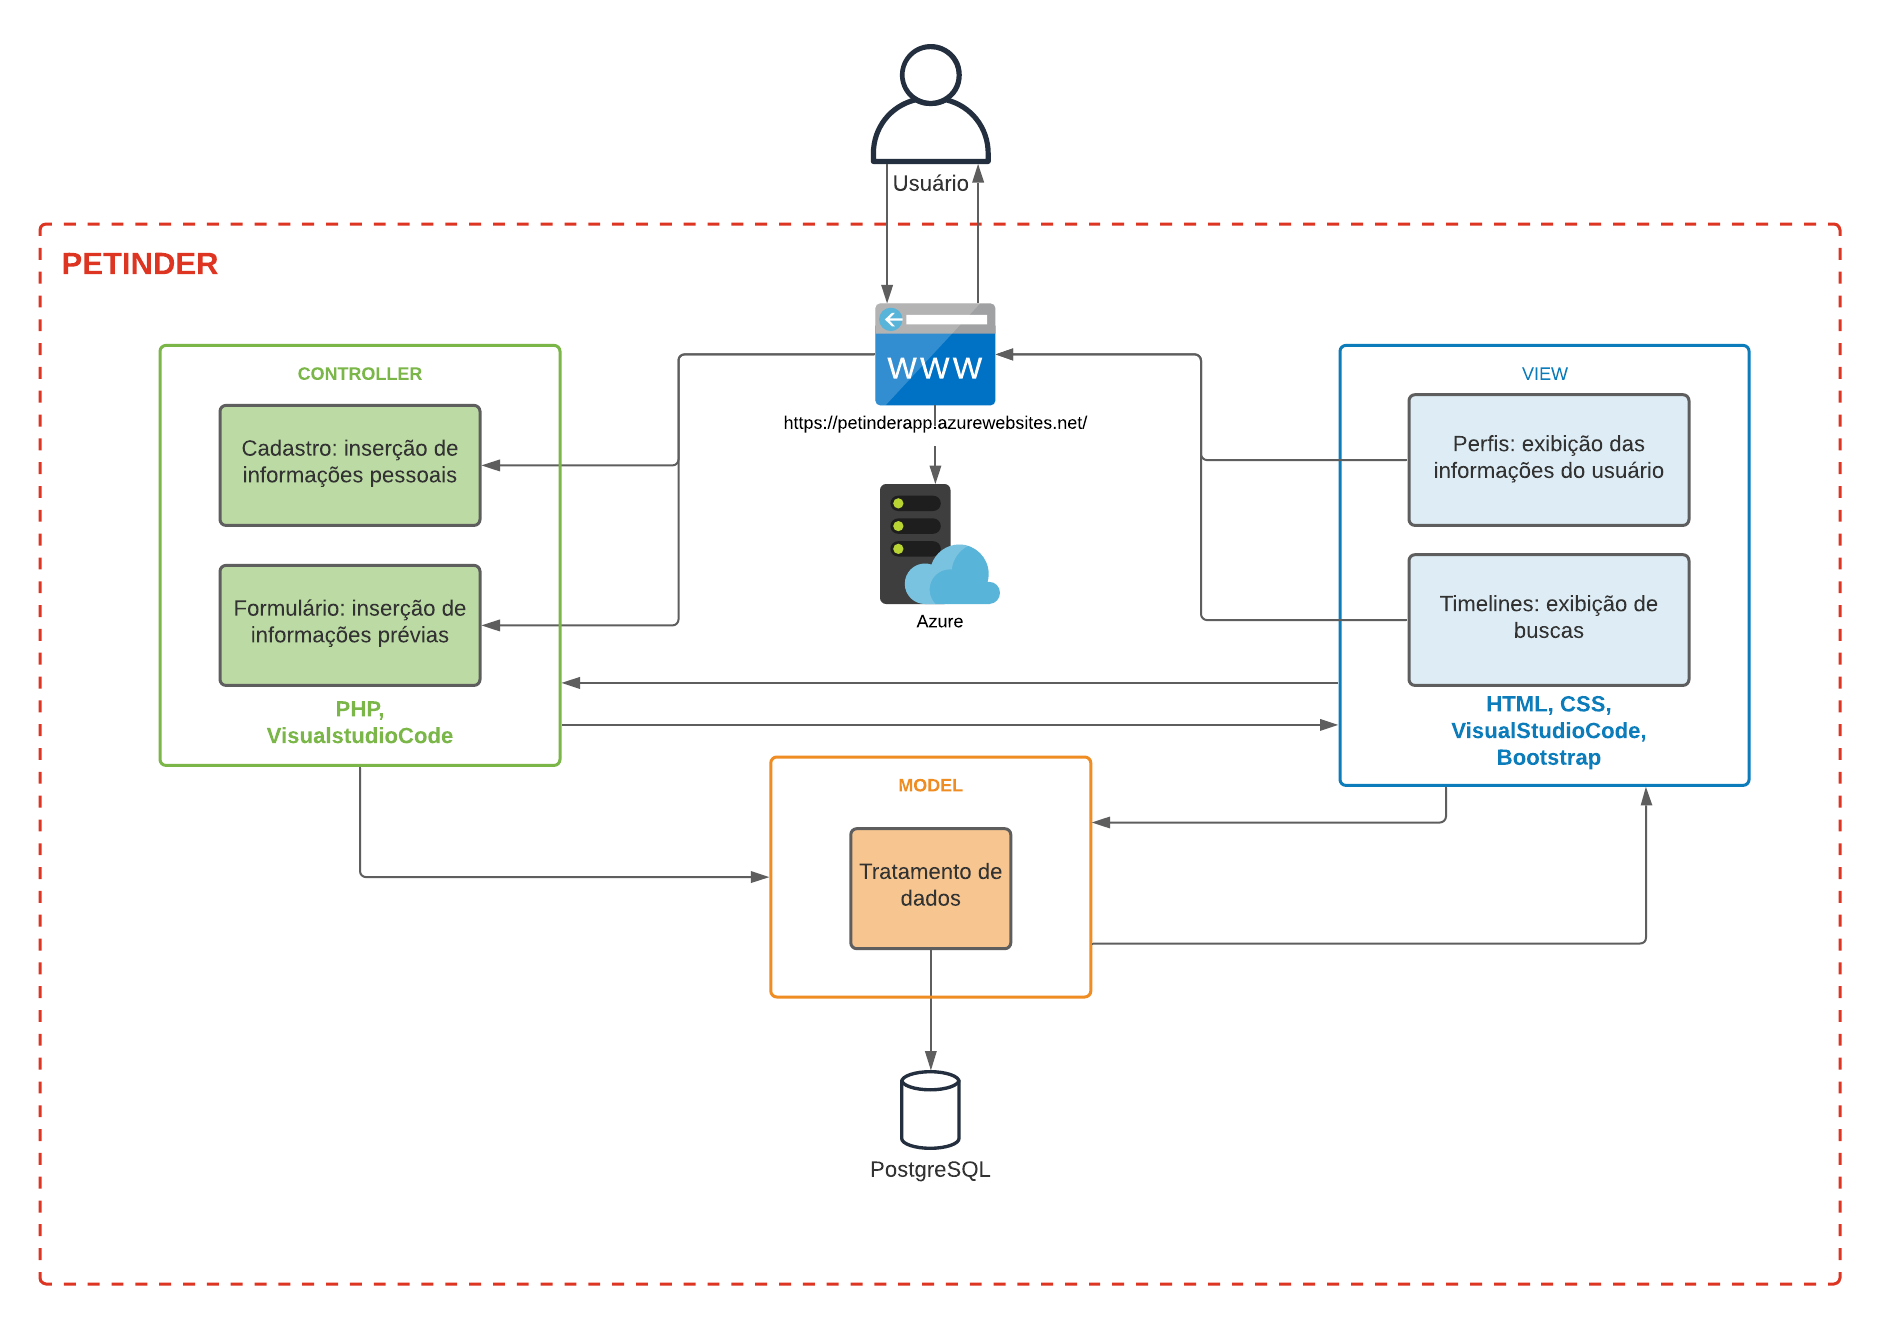
\includegraphics[width=1\textwidth,pagecommand=\chapter{}]{imagens/DiagramaDeArquitetura_PETINDER.png}
    \label{diagrama-casos}
    \fonte{Elaborado pelos autores}
\end{figure}

\begin{figure}[htb]
\chapter{Teste de confiabilidade SSL}
\label{teste-ssl}
    \centering
    \caption{Certificado SSL nota A}
    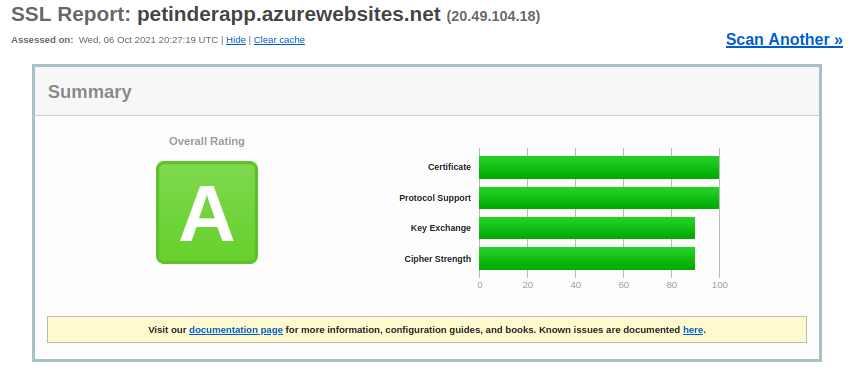
\includegraphics[scale=0.65,angle=90]{imagens/certificado_ssl.png}
    \label{teste-ssl-img}
    \fonte{Elaborado pelos autores}
\end{figure}

\chapter{Testes Automatizados}
\label{testes}

\begin{figure}[!htbp]
\begin{flushleft}
    \section{Teste - Animais mais próximos}
\end{flushleft}
    \centering
    \caption{Teste Animais mais próximos}
    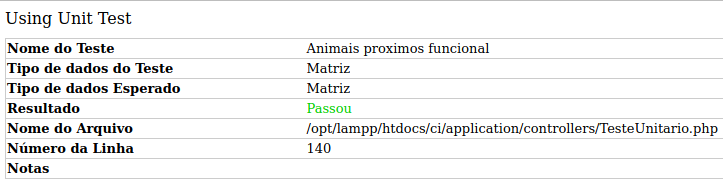
\includegraphics[width=0.9\textwidth,pagecommand=\chapter{}]{imagens/test_distancia.png}
    \label{teste-distancia}
    \fonte{Elaborado pelos autores}
\end{figure}

\begin{figure}[htb]
    \centering
    \caption{\label{fig_timeline}Plano de Testes - Animais mais próximos}
	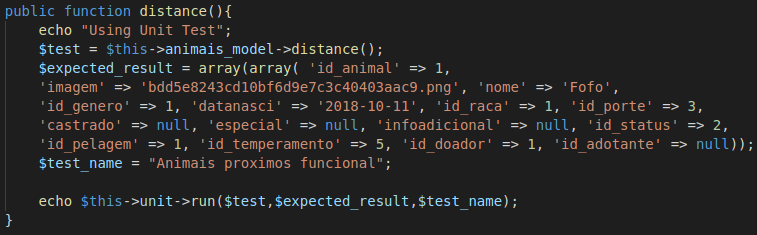
\includegraphics[width=1\textwidth]{imagens/cod_teste_distance.png}
	\fonte{Elaborada pelos autores}
\end{figure}

\begin{figure}[!htbp]
\begin{flushleft}
    \section{Teste - Deletar Animal}
\end{flushleft}
    \centering
    \caption{Teste Deletar Animal}
    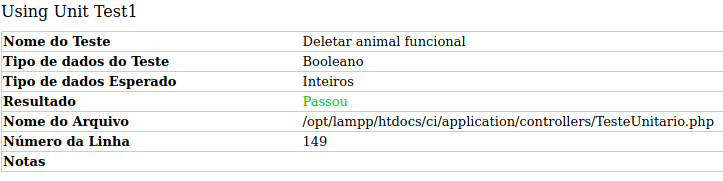
\includegraphics[width=1\textwidth,pagecommand=\chapter{}]{imagens/teste_deletar_animal.png}
    \label{teste-deletar-animal}
    \fonte{Elaborado pelos autores}
\end{figure}

\begin{figure}[htb]
    \centering
    \caption{\label{fig_timeline}Plano de Testes - Deletar Animal}
	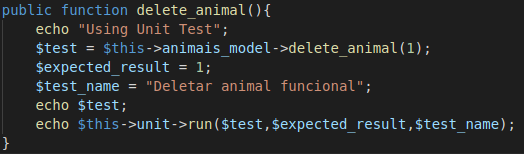
\includegraphics[width=1\textwidth]{imagens/cod_teste_delete_animal.png}
	\fonte{Elaborada pelos autores}
\end{figure}

\begin{figure}[!htbp]
\begin{flushleft}
    \section{Teste - Combinação Perfeita}
\end{flushleft}
    \centering
    \caption{Teste Combinação Perfeita}
    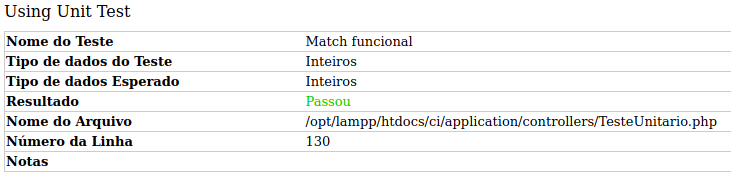
\includegraphics[width=1\textwidth,pagecommand=\chapter{}]{imagens/teste_match.png}
    \label{teste-match}
    \fonte{Elaborado pelos autores}
\end{figure}

\begin{figure}[htb]
    \centering
    \caption{\label{fig_timeline}Plano de Testes - Combinação Perfeita}
	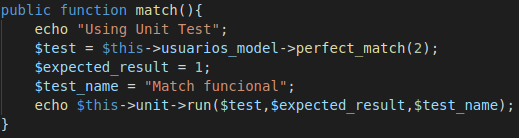
\includegraphics[width=1\textwidth]{imagens/cod_teste_match.png}
	\fonte{Elaborada pelos autores}
\end{figure}

\begin{figure}[!htbp]
\begin{flushleft}
    \section{Teste - Denúncia}
\end{flushleft}
    \centering
    \caption{Teste Denúncia}
    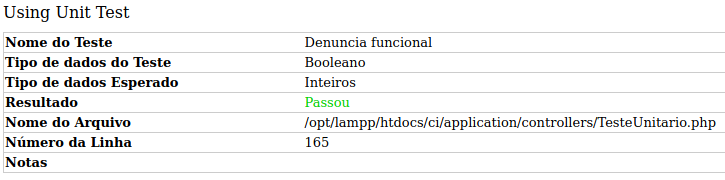
\includegraphics[width=1\textwidth,pagecommand=\chapter{}]{imagens/teste_denuncia.png}
    \label{teste-denuncia}
    \fonte{Elaborado pelos autores}
\end{figure}

\begin{figure}[htb]
    \centering
    \caption{\label{fig_timeline}Plano de Testes - Denúncia}
	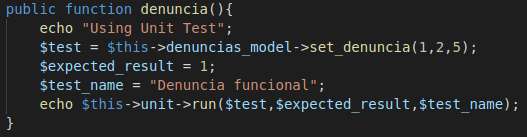
\includegraphics[width=1\textwidth]{imagens/cod_teste_denuncia.png}
	\fonte{Elaborada pelos autores}
\end{figure}

\begin{figure}[!htbp]
\begin{flushleft}
    \section{Teste - Espécie}
\end{flushleft}
    \centering
    \caption{Teste Espécie}
    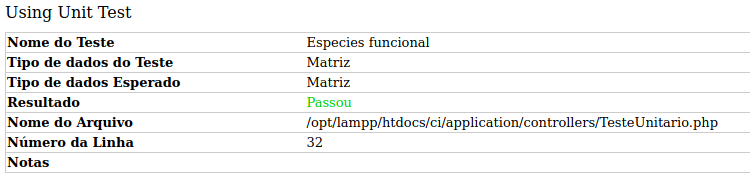
\includegraphics[width=1\textwidth,pagecommand=\chapter{}]{imagens/teste_especie.png}
    \label{teste-especie}
    \fonte{Elaborado pelos autores}
\end{figure}

\begin{figure}[htb]
    \centering
    \caption{\label{fig_timeline}Plano de Testes - Espécie}
	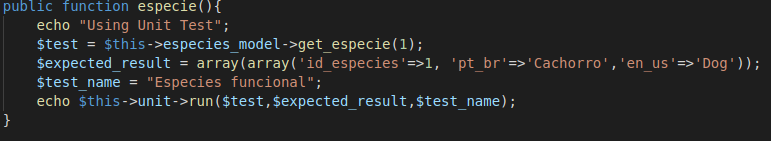
\includegraphics[width=1\textwidth]{imagens/cod_teste_especie.png}
	\fonte{Elaborada pelos autores}
\end{figure}

\begin{figure}[!htbp]
\begin{flushleft}
    \section{Teste - Gênero}
\end{flushleft}
    \centering
    \caption{Teste Gênero}
    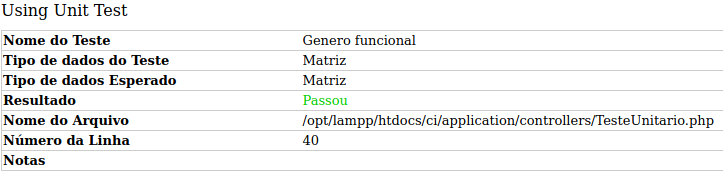
\includegraphics[width=1\textwidth,pagecommand=\chapter{}]{imagens/teste_genero.png}
    \label{teste-genero}
    \fonte{Elaborado pelos autores}
\end{figure}

\begin{figure}[htb]
    \centering
    \caption{\label{fig_timeline}Plano de Testes - Gênero}
	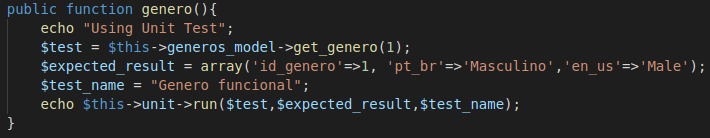
\includegraphics[width=1\textwidth]{imagens/cod_teste_genero.png}
	\fonte{Elaborada pelos autores}
\end{figure}

\begin{figure}[!htbp]
\begin{flushleft}
    \section{Teste - Horas Sozinho}
\end{flushleft}
    \centering
    \caption{Teste Horas Sozinho}
    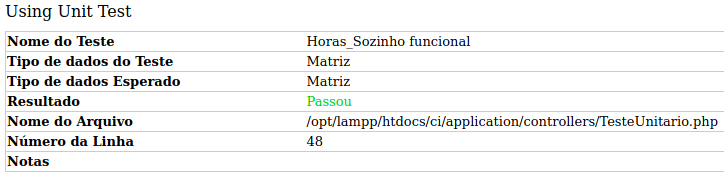
\includegraphics[width=1\textwidth,pagecommand=\chapter{}]{imagens/teste_horassozinho.png}
    \label{teste-horas-so}
    \fonte{Elaborado pelos autores}
\end{figure}

\begin{figure}[htb]
    \centering
    \caption{\label{fig_timeline}Plano de Testes - Horas Sozinho}
	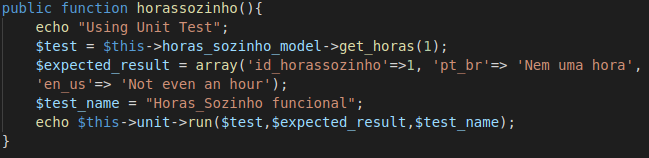
\includegraphics[width=1\textwidth]{imagens/cod_teste_horassozinho.png}
	\fonte{Elaborada pelos autores}
\end{figure}

\begin{figure}[!htbp]
\begin{flushleft}
    \section{Teste - Login}
\end{flushleft}
    \centering
    \caption{Teste Login}
    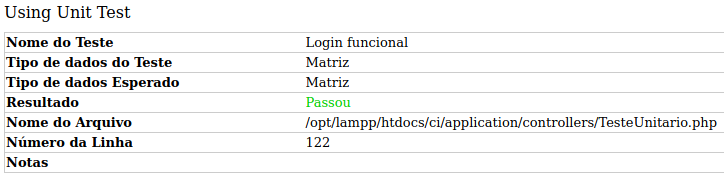
\includegraphics[width=1\textwidth,pagecommand=\chapter{}]{imagens/teste_login.png}
    \label{teste-login}
    \fonte{Elaborado pelos autores}
\end{figure}

\begin{figure}[htb]
    \centering
    \caption{\label{fig_timeline}Plano de Testes - Login}
	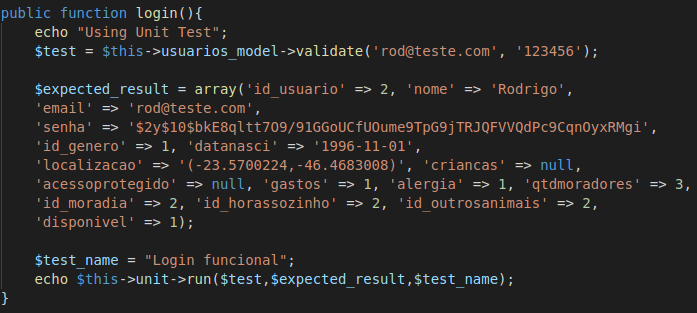
\includegraphics[width=1\textwidth]{imagens/cod_teste_login.png}
	\fonte{Elaborada pelos autores}
\end{figure}

\begin{figure}[!htbp]
\begin{flushleft}
    \section{Teste - Moradia}
\end{flushleft}
    \centering
    \caption{Teste Moradia}
    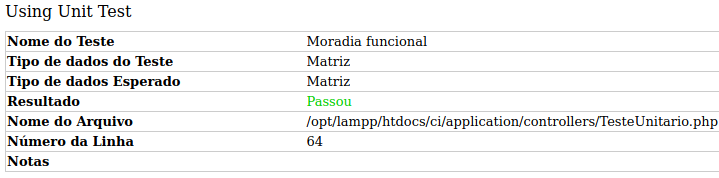
\includegraphics[width=1\textwidth,pagecommand=\chapter{}]{imagens/teste_moradia.png}
    \label{teste-moradia}
    \fonte{Elaborado pelos autores}
\end{figure}

\begin{figure}[htb]
    \centering
    \caption{\label{fig_timeline}Plano de Testes - Moradia}
	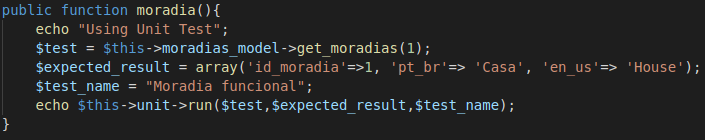
\includegraphics[width=1\textwidth]{imagens/cod_teste_moradia.png}
	\fonte{Elaborada pelos autores}
\end{figure}

\begin{figure}[!htbp]
\begin{flushleft}
    \section{Teste - Motivo Denúncia}
\end{flushleft}
    \centering 
    \caption{Teste Motivo Denúncia}
    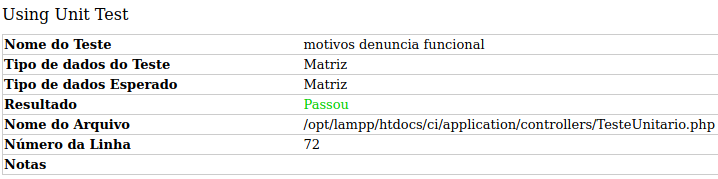
\includegraphics[width=1\textwidth,pagecommand=\chapter{}]{imagens/teste_motivos_denuncia.png}
    \label{teste-motivo}
    \fonte{Elaborado pelos autores}
\end{figure}

\begin{figure}[htb]
    \centering
    \caption{\label{fig_timeline}Plano de Testes - Motivo Denúncia}
	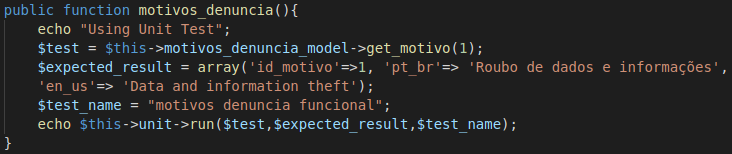
\includegraphics[width=1\textwidth]{imagens/cod_teste_motivos_denuncia.png}
	\fonte{Elaborada pelos autores}
\end{figure}

\begin{figure}[!htbp]
\begin{flushleft}
    \section{Teste - Mudar Status da Mensagem}
\end{flushleft}
    \centering
    \caption{Teste Mudar Status da Mensagem}
    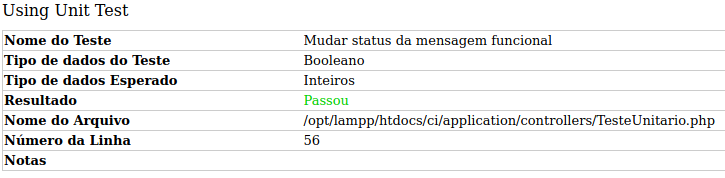
\includegraphics[width=1\textwidth,pagecommand=\chapter{}]{imagens/teste_msg.png}
    \label{teste-mensagem}
    \fonte{Elaborado pelos autores}
\end{figure}

\begin{figure}[htb]
    \centering
    \caption{\label{fig_timeline}Plano de Testes - Mudar Status da Mensagem}
	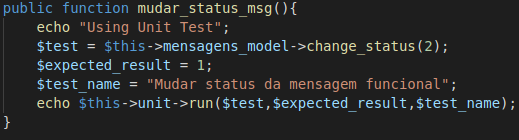
\includegraphics[width=1\textwidth]{imagens/cod_teste_mudar_status.png}
	\fonte{Elaborada pelos autores}
\end{figure}

\begin{figure}[!htbp]
\begin{flushleft}
    \section{Teste - Outros Animais}
\end{flushleft}
    \centering
    \caption{Teste Outros Animais}
    \includegraphics[width=1\textwidth,pagecommand=\chapter{}]{imagens/teste_especie.png}
    \label{teste-outros-animais}
    \fonte{Elaborado pelos autores}
\end{figure}

\begin{figure}[htb]
    \centering
    \caption{\label{fig_timeline}Plano de Testes - Outros Animais}
	\includegraphics[width=1\textwidth]{imagens/cod_teste_outrosanimais.png}
	\fonte{Elaborada pelos autores}
\end{figure}

\begin{figure}[!htbp]
\begin{flushleft}
    \section{Teste - Pelagem}
\end{flushleft}
    \centering
    \caption{Teste Pelagem}
    \includegraphics[width=1\textwidth,pagecommand=\chapter{}]{imagens/teste_pelagem.png}
    \label{teste-pelagem}
    \fonte{Elaborado pelos autores}
\end{figure}

\begin{figure}[htb]
    \centering
    \caption{\label{fig_timeline}Plano de Testes - Pelagem}
	\includegraphics[width=1\textwidth]{imagens/cod_teste_pelagem.png}
	\fonte{Elaborada pelos autores}
\end{figure}

\begin{figure}[!htbp]
\begin{flushleft}
    \section{Teste - Porte}
\end{flushleft}
    \centering
    \caption{Teste Porte}
    \includegraphics[width=1\textwidth,pagecommand=\chapter{}]{imagens/teste_porte.png}
    \label{teste-porte}
    \fonte{Elaborado pelos autores}
\end{figure}

\begin{figure}[htb]
    \centering
    \caption{\label{fig_timeline}Plano de Testes - Porte}
	\includegraphics[width=1\textwidth]{imagens/cod_teste_porte.png}
	\fonte{Elaborada pelos autores}
\end{figure}

\begin{figure}[!htbp]
\begin{flushleft}
    \section{Teste - Match}
\end{flushleft}
    \centering
    \caption{Teste Match}
    \includegraphics[width=1\textwidth,pagecommand=\chapter{}]{imagens/teste_set_match.png}
    \label{teste-set-match}
    \fonte{Elaborado pelos autores}
\end{figure}

\begin{figure}[htb]
    \centering
    \caption{\label{fig_timeline}Plano de Testes - Match}
	\includegraphics[width=1\textwidth]{imagens/cod_teste_match.png}
	\fonte{Elaborada pelos autores}
\end{figure}

\begin{figure}[!htbp]
\begin{flushleft}
    \section{Teste - Status do animal}
\end{flushleft}
    \centering
    \caption{Teste Status do animal}
    \includegraphics[width=1\textwidth,pagecommand=\chapter{}]{imagens/teste_status.png}
    \label{teste-status}
    \fonte{Elaborado pelos autores}
\end{figure}

\begin{figure}[htb]
    \centering
    \caption{\label{fig_timeline}Plano de Testes - Status do animal}
	\includegraphics[width=1\textwidth]{imagens/cod_teste_status.png}
	\fonte{Elaborada pelos autores}
\end{figure}

\begin{figure}[!htbp]
\begin{flushleft}
    \section{Teste - Temperamento}
\end{flushleft}
    \centering
    \caption{Teste Temperamento}
    \includegraphics[width=1\textwidth,pagecommand=\chapter{}]{imagens/teste_temperamento.png}
    \label{teste-temperamento}
    \fonte{Elaborado pelos autores}
\end{figure}

\begin{figure}[htb]
    \centering
    \caption{\label{fig_timeline}Plano de Testes - Temperamento}
	\includegraphics[width=1\textwidth]{imagens/cod_teste_temperamento.png}
	\fonte{Elaborada pelos autores}
\end{figure}

% ---
\end{apendicesenv}
% ---




%% ----------------------------------------------------------
% Anexos
% Documentos gerados por outros autores
% ----------------------------------------------------------

% ---
% Inicia os anexos
% ---
\begin{anexosenv}
\anexos
% Imprime uma página indicando o início dos anexos
\partanexos
% ---
\chapter{Manual todonotes(parcial)}
\label{manual-todonotes}
% ---
\index{pdf}
% se pages = "-"  fica com arquivo completo
%\includepdf[pages=1-3,scale=0.8,frame=true,pagecommand={}]{anexos/PropostaInicial.pdf}

% ---
% Para incluir sem gerar a quebra de página inicial no anexo
%\includepdf[pages=1,scale=0.7,frame=true,pagecommand=\chapter{Manual pdfpages(parcial)}\label{manual-pdfpages}]{}

\end{anexosenv}



%---------------------------------------------------------------------
% INDICE REMISSIVO - Quando necessário 
% As palavras indexadas devem ser definidas com \index{} no texto
%---------------------------------------------------------------------
\phantompart
\printindex
\todonum[inline]{remover indice remissivo se não for necessário}

%---------------------------------------------------------------------

\end{document}